
% Default to the notebook output style

    


% Inherit from the specified cell style.




    
\documentclass[11pt]{article}

    
    
    \usepackage[T1]{fontenc}
    % Nicer default font (+ math font) than Computer Modern for most use cases
    \usepackage{mathpazo}

    % Basic figure setup, for now with no caption control since it's done
    % automatically by Pandoc (which extracts ![](path) syntax from Markdown).
    \usepackage{graphicx}
    % We will generate all images so they have a width \maxwidth. This means
    % that they will get their normal width if they fit onto the page, but
    % are scaled down if they would overflow the margins.
    \makeatletter
    \def\maxwidth{\ifdim\Gin@nat@width>\linewidth\linewidth
    \else\Gin@nat@width\fi}
    \makeatother
    \let\Oldincludegraphics\includegraphics
    % Set max figure width to be 80% of text width, for now hardcoded.
    \renewcommand{\includegraphics}[1]{\Oldincludegraphics[width=.8\maxwidth]{#1}}
    % Ensure that by default, figures have no caption (until we provide a
    % proper Figure object with a Caption API and a way to capture that
    % in the conversion process - todo).
    \usepackage{caption}
    \DeclareCaptionLabelFormat{nolabel}{}
    \captionsetup{labelformat=nolabel}

    \usepackage{adjustbox} % Used to constrain images to a maximum size 
    \usepackage{xcolor} % Allow colors to be defined
    \usepackage{enumerate} % Needed for markdown enumerations to work
    \usepackage{geometry} % Used to adjust the document margins
    \usepackage{amsmath} % Equations
    \usepackage{amssymb} % Equations
    \usepackage{textcomp} % defines textquotesingle
    % Hack from http://tex.stackexchange.com/a/47451/13684:
    \AtBeginDocument{%
        \def\PYZsq{\textquotesingle}% Upright quotes in Pygmentized code
    }
    \usepackage{upquote} % Upright quotes for verbatim code
    \usepackage{eurosym} % defines \euro
    \usepackage[mathletters]{ucs} % Extended unicode (utf-8) support
    \usepackage[utf8x]{inputenc} % Allow utf-8 characters in the tex document
    \usepackage{fancyvrb} % verbatim replacement that allows latex
    \usepackage{grffile} % extends the file name processing of package graphics 
                         % to support a larger range 
    % The hyperref package gives us a pdf with properly built
    % internal navigation ('pdf bookmarks' for the table of contents,
    % internal cross-reference links, web links for URLs, etc.)
    \usepackage{hyperref}
    \usepackage{longtable} % longtable support required by pandoc >1.10
    \usepackage{booktabs}  % table support for pandoc > 1.12.2
    \usepackage[inline]{enumitem} % IRkernel/repr support (it uses the enumerate* environment)
    \usepackage[normalem]{ulem} % ulem is needed to support strikethroughs (\sout)
                                % normalem makes italics be italics, not underlines
    

    
    
    % Colors for the hyperref package
    \definecolor{urlcolor}{rgb}{0,.145,.698}
    \definecolor{linkcolor}{rgb}{.71,0.21,0.01}
    \definecolor{citecolor}{rgb}{.12,.54,.11}

    % ANSI colors
    \definecolor{ansi-black}{HTML}{3E424D}
    \definecolor{ansi-black-intense}{HTML}{282C36}
    \definecolor{ansi-red}{HTML}{E75C58}
    \definecolor{ansi-red-intense}{HTML}{B22B31}
    \definecolor{ansi-green}{HTML}{00A250}
    \definecolor{ansi-green-intense}{HTML}{007427}
    \definecolor{ansi-yellow}{HTML}{DDB62B}
    \definecolor{ansi-yellow-intense}{HTML}{B27D12}
    \definecolor{ansi-blue}{HTML}{208FFB}
    \definecolor{ansi-blue-intense}{HTML}{0065CA}
    \definecolor{ansi-magenta}{HTML}{D160C4}
    \definecolor{ansi-magenta-intense}{HTML}{A03196}
    \definecolor{ansi-cyan}{HTML}{60C6C8}
    \definecolor{ansi-cyan-intense}{HTML}{258F8F}
    \definecolor{ansi-white}{HTML}{C5C1B4}
    \definecolor{ansi-white-intense}{HTML}{A1A6B2}

    % commands and environments needed by pandoc snippets
    % extracted from the output of `pandoc -s`
    \providecommand{\tightlist}{%
      \setlength{\itemsep}{0pt}\setlength{\parskip}{0pt}}
    \DefineVerbatimEnvironment{Highlighting}{Verbatim}{commandchars=\\\{\}}
    % Add ',fontsize=\small' for more characters per line
    \newenvironment{Shaded}{}{}
    \newcommand{\KeywordTok}[1]{\textcolor[rgb]{0.00,0.44,0.13}{\textbf{{#1}}}}
    \newcommand{\DataTypeTok}[1]{\textcolor[rgb]{0.56,0.13,0.00}{{#1}}}
    \newcommand{\DecValTok}[1]{\textcolor[rgb]{0.25,0.63,0.44}{{#1}}}
    \newcommand{\BaseNTok}[1]{\textcolor[rgb]{0.25,0.63,0.44}{{#1}}}
    \newcommand{\FloatTok}[1]{\textcolor[rgb]{0.25,0.63,0.44}{{#1}}}
    \newcommand{\CharTok}[1]{\textcolor[rgb]{0.25,0.44,0.63}{{#1}}}
    \newcommand{\StringTok}[1]{\textcolor[rgb]{0.25,0.44,0.63}{{#1}}}
    \newcommand{\CommentTok}[1]{\textcolor[rgb]{0.38,0.63,0.69}{\textit{{#1}}}}
    \newcommand{\OtherTok}[1]{\textcolor[rgb]{0.00,0.44,0.13}{{#1}}}
    \newcommand{\AlertTok}[1]{\textcolor[rgb]{1.00,0.00,0.00}{\textbf{{#1}}}}
    \newcommand{\FunctionTok}[1]{\textcolor[rgb]{0.02,0.16,0.49}{{#1}}}
    \newcommand{\RegionMarkerTok}[1]{{#1}}
    \newcommand{\ErrorTok}[1]{\textcolor[rgb]{1.00,0.00,0.00}{\textbf{{#1}}}}
    \newcommand{\NormalTok}[1]{{#1}}
    
    % Additional commands for more recent versions of Pandoc
    \newcommand{\ConstantTok}[1]{\textcolor[rgb]{0.53,0.00,0.00}{{#1}}}
    \newcommand{\SpecialCharTok}[1]{\textcolor[rgb]{0.25,0.44,0.63}{{#1}}}
    \newcommand{\VerbatimStringTok}[1]{\textcolor[rgb]{0.25,0.44,0.63}{{#1}}}
    \newcommand{\SpecialStringTok}[1]{\textcolor[rgb]{0.73,0.40,0.53}{{#1}}}
    \newcommand{\ImportTok}[1]{{#1}}
    \newcommand{\DocumentationTok}[1]{\textcolor[rgb]{0.73,0.13,0.13}{\textit{{#1}}}}
    \newcommand{\AnnotationTok}[1]{\textcolor[rgb]{0.38,0.63,0.69}{\textbf{\textit{{#1}}}}}
    \newcommand{\CommentVarTok}[1]{\textcolor[rgb]{0.38,0.63,0.69}{\textbf{\textit{{#1}}}}}
    \newcommand{\VariableTok}[1]{\textcolor[rgb]{0.10,0.09,0.49}{{#1}}}
    \newcommand{\ControlFlowTok}[1]{\textcolor[rgb]{0.00,0.44,0.13}{\textbf{{#1}}}}
    \newcommand{\OperatorTok}[1]{\textcolor[rgb]{0.40,0.40,0.40}{{#1}}}
    \newcommand{\BuiltInTok}[1]{{#1}}
    \newcommand{\ExtensionTok}[1]{{#1}}
    \newcommand{\PreprocessorTok}[1]{\textcolor[rgb]{0.74,0.48,0.00}{{#1}}}
    \newcommand{\AttributeTok}[1]{\textcolor[rgb]{0.49,0.56,0.16}{{#1}}}
    \newcommand{\InformationTok}[1]{\textcolor[rgb]{0.38,0.63,0.69}{\textbf{\textit{{#1}}}}}
    \newcommand{\WarningTok}[1]{\textcolor[rgb]{0.38,0.63,0.69}{\textbf{\textit{{#1}}}}}
    
    
    % Define a nice break command that doesn't care if a line doesn't already
    % exist.
    \def\br{\hspace*{\fill} \\* }
    % Math Jax compatability definitions
    \def\gt{>}
    \def\lt{<}
    % Document parameters
    \title{Lesson03C\_Keras\_API}
    
    
    

    % Pygments definitions
    
\makeatletter
\def\PY@reset{\let\PY@it=\relax \let\PY@bf=\relax%
    \let\PY@ul=\relax \let\PY@tc=\relax%
    \let\PY@bc=\relax \let\PY@ff=\relax}
\def\PY@tok#1{\csname PY@tok@#1\endcsname}
\def\PY@toks#1+{\ifx\relax#1\empty\else%
    \PY@tok{#1}\expandafter\PY@toks\fi}
\def\PY@do#1{\PY@bc{\PY@tc{\PY@ul{%
    \PY@it{\PY@bf{\PY@ff{#1}}}}}}}
\def\PY#1#2{\PY@reset\PY@toks#1+\relax+\PY@do{#2}}

\expandafter\def\csname PY@tok@w\endcsname{\def\PY@tc##1{\textcolor[rgb]{0.73,0.73,0.73}{##1}}}
\expandafter\def\csname PY@tok@c\endcsname{\let\PY@it=\textit\def\PY@tc##1{\textcolor[rgb]{0.25,0.50,0.50}{##1}}}
\expandafter\def\csname PY@tok@cp\endcsname{\def\PY@tc##1{\textcolor[rgb]{0.74,0.48,0.00}{##1}}}
\expandafter\def\csname PY@tok@k\endcsname{\let\PY@bf=\textbf\def\PY@tc##1{\textcolor[rgb]{0.00,0.50,0.00}{##1}}}
\expandafter\def\csname PY@tok@kp\endcsname{\def\PY@tc##1{\textcolor[rgb]{0.00,0.50,0.00}{##1}}}
\expandafter\def\csname PY@tok@kt\endcsname{\def\PY@tc##1{\textcolor[rgb]{0.69,0.00,0.25}{##1}}}
\expandafter\def\csname PY@tok@o\endcsname{\def\PY@tc##1{\textcolor[rgb]{0.40,0.40,0.40}{##1}}}
\expandafter\def\csname PY@tok@ow\endcsname{\let\PY@bf=\textbf\def\PY@tc##1{\textcolor[rgb]{0.67,0.13,1.00}{##1}}}
\expandafter\def\csname PY@tok@nb\endcsname{\def\PY@tc##1{\textcolor[rgb]{0.00,0.50,0.00}{##1}}}
\expandafter\def\csname PY@tok@nf\endcsname{\def\PY@tc##1{\textcolor[rgb]{0.00,0.00,1.00}{##1}}}
\expandafter\def\csname PY@tok@nc\endcsname{\let\PY@bf=\textbf\def\PY@tc##1{\textcolor[rgb]{0.00,0.00,1.00}{##1}}}
\expandafter\def\csname PY@tok@nn\endcsname{\let\PY@bf=\textbf\def\PY@tc##1{\textcolor[rgb]{0.00,0.00,1.00}{##1}}}
\expandafter\def\csname PY@tok@ne\endcsname{\let\PY@bf=\textbf\def\PY@tc##1{\textcolor[rgb]{0.82,0.25,0.23}{##1}}}
\expandafter\def\csname PY@tok@nv\endcsname{\def\PY@tc##1{\textcolor[rgb]{0.10,0.09,0.49}{##1}}}
\expandafter\def\csname PY@tok@no\endcsname{\def\PY@tc##1{\textcolor[rgb]{0.53,0.00,0.00}{##1}}}
\expandafter\def\csname PY@tok@nl\endcsname{\def\PY@tc##1{\textcolor[rgb]{0.63,0.63,0.00}{##1}}}
\expandafter\def\csname PY@tok@ni\endcsname{\let\PY@bf=\textbf\def\PY@tc##1{\textcolor[rgb]{0.60,0.60,0.60}{##1}}}
\expandafter\def\csname PY@tok@na\endcsname{\def\PY@tc##1{\textcolor[rgb]{0.49,0.56,0.16}{##1}}}
\expandafter\def\csname PY@tok@nt\endcsname{\let\PY@bf=\textbf\def\PY@tc##1{\textcolor[rgb]{0.00,0.50,0.00}{##1}}}
\expandafter\def\csname PY@tok@nd\endcsname{\def\PY@tc##1{\textcolor[rgb]{0.67,0.13,1.00}{##1}}}
\expandafter\def\csname PY@tok@s\endcsname{\def\PY@tc##1{\textcolor[rgb]{0.73,0.13,0.13}{##1}}}
\expandafter\def\csname PY@tok@sd\endcsname{\let\PY@it=\textit\def\PY@tc##1{\textcolor[rgb]{0.73,0.13,0.13}{##1}}}
\expandafter\def\csname PY@tok@si\endcsname{\let\PY@bf=\textbf\def\PY@tc##1{\textcolor[rgb]{0.73,0.40,0.53}{##1}}}
\expandafter\def\csname PY@tok@se\endcsname{\let\PY@bf=\textbf\def\PY@tc##1{\textcolor[rgb]{0.73,0.40,0.13}{##1}}}
\expandafter\def\csname PY@tok@sr\endcsname{\def\PY@tc##1{\textcolor[rgb]{0.73,0.40,0.53}{##1}}}
\expandafter\def\csname PY@tok@ss\endcsname{\def\PY@tc##1{\textcolor[rgb]{0.10,0.09,0.49}{##1}}}
\expandafter\def\csname PY@tok@sx\endcsname{\def\PY@tc##1{\textcolor[rgb]{0.00,0.50,0.00}{##1}}}
\expandafter\def\csname PY@tok@m\endcsname{\def\PY@tc##1{\textcolor[rgb]{0.40,0.40,0.40}{##1}}}
\expandafter\def\csname PY@tok@gh\endcsname{\let\PY@bf=\textbf\def\PY@tc##1{\textcolor[rgb]{0.00,0.00,0.50}{##1}}}
\expandafter\def\csname PY@tok@gu\endcsname{\let\PY@bf=\textbf\def\PY@tc##1{\textcolor[rgb]{0.50,0.00,0.50}{##1}}}
\expandafter\def\csname PY@tok@gd\endcsname{\def\PY@tc##1{\textcolor[rgb]{0.63,0.00,0.00}{##1}}}
\expandafter\def\csname PY@tok@gi\endcsname{\def\PY@tc##1{\textcolor[rgb]{0.00,0.63,0.00}{##1}}}
\expandafter\def\csname PY@tok@gr\endcsname{\def\PY@tc##1{\textcolor[rgb]{1.00,0.00,0.00}{##1}}}
\expandafter\def\csname PY@tok@ge\endcsname{\let\PY@it=\textit}
\expandafter\def\csname PY@tok@gs\endcsname{\let\PY@bf=\textbf}
\expandafter\def\csname PY@tok@gp\endcsname{\let\PY@bf=\textbf\def\PY@tc##1{\textcolor[rgb]{0.00,0.00,0.50}{##1}}}
\expandafter\def\csname PY@tok@go\endcsname{\def\PY@tc##1{\textcolor[rgb]{0.53,0.53,0.53}{##1}}}
\expandafter\def\csname PY@tok@gt\endcsname{\def\PY@tc##1{\textcolor[rgb]{0.00,0.27,0.87}{##1}}}
\expandafter\def\csname PY@tok@err\endcsname{\def\PY@bc##1{\setlength{\fboxsep}{0pt}\fcolorbox[rgb]{1.00,0.00,0.00}{1,1,1}{\strut ##1}}}
\expandafter\def\csname PY@tok@kc\endcsname{\let\PY@bf=\textbf\def\PY@tc##1{\textcolor[rgb]{0.00,0.50,0.00}{##1}}}
\expandafter\def\csname PY@tok@kd\endcsname{\let\PY@bf=\textbf\def\PY@tc##1{\textcolor[rgb]{0.00,0.50,0.00}{##1}}}
\expandafter\def\csname PY@tok@kn\endcsname{\let\PY@bf=\textbf\def\PY@tc##1{\textcolor[rgb]{0.00,0.50,0.00}{##1}}}
\expandafter\def\csname PY@tok@kr\endcsname{\let\PY@bf=\textbf\def\PY@tc##1{\textcolor[rgb]{0.00,0.50,0.00}{##1}}}
\expandafter\def\csname PY@tok@bp\endcsname{\def\PY@tc##1{\textcolor[rgb]{0.00,0.50,0.00}{##1}}}
\expandafter\def\csname PY@tok@fm\endcsname{\def\PY@tc##1{\textcolor[rgb]{0.00,0.00,1.00}{##1}}}
\expandafter\def\csname PY@tok@vc\endcsname{\def\PY@tc##1{\textcolor[rgb]{0.10,0.09,0.49}{##1}}}
\expandafter\def\csname PY@tok@vg\endcsname{\def\PY@tc##1{\textcolor[rgb]{0.10,0.09,0.49}{##1}}}
\expandafter\def\csname PY@tok@vi\endcsname{\def\PY@tc##1{\textcolor[rgb]{0.10,0.09,0.49}{##1}}}
\expandafter\def\csname PY@tok@vm\endcsname{\def\PY@tc##1{\textcolor[rgb]{0.10,0.09,0.49}{##1}}}
\expandafter\def\csname PY@tok@sa\endcsname{\def\PY@tc##1{\textcolor[rgb]{0.73,0.13,0.13}{##1}}}
\expandafter\def\csname PY@tok@sb\endcsname{\def\PY@tc##1{\textcolor[rgb]{0.73,0.13,0.13}{##1}}}
\expandafter\def\csname PY@tok@sc\endcsname{\def\PY@tc##1{\textcolor[rgb]{0.73,0.13,0.13}{##1}}}
\expandafter\def\csname PY@tok@dl\endcsname{\def\PY@tc##1{\textcolor[rgb]{0.73,0.13,0.13}{##1}}}
\expandafter\def\csname PY@tok@s2\endcsname{\def\PY@tc##1{\textcolor[rgb]{0.73,0.13,0.13}{##1}}}
\expandafter\def\csname PY@tok@sh\endcsname{\def\PY@tc##1{\textcolor[rgb]{0.73,0.13,0.13}{##1}}}
\expandafter\def\csname PY@tok@s1\endcsname{\def\PY@tc##1{\textcolor[rgb]{0.73,0.13,0.13}{##1}}}
\expandafter\def\csname PY@tok@mb\endcsname{\def\PY@tc##1{\textcolor[rgb]{0.40,0.40,0.40}{##1}}}
\expandafter\def\csname PY@tok@mf\endcsname{\def\PY@tc##1{\textcolor[rgb]{0.40,0.40,0.40}{##1}}}
\expandafter\def\csname PY@tok@mh\endcsname{\def\PY@tc##1{\textcolor[rgb]{0.40,0.40,0.40}{##1}}}
\expandafter\def\csname PY@tok@mi\endcsname{\def\PY@tc##1{\textcolor[rgb]{0.40,0.40,0.40}{##1}}}
\expandafter\def\csname PY@tok@il\endcsname{\def\PY@tc##1{\textcolor[rgb]{0.40,0.40,0.40}{##1}}}
\expandafter\def\csname PY@tok@mo\endcsname{\def\PY@tc##1{\textcolor[rgb]{0.40,0.40,0.40}{##1}}}
\expandafter\def\csname PY@tok@ch\endcsname{\let\PY@it=\textit\def\PY@tc##1{\textcolor[rgb]{0.25,0.50,0.50}{##1}}}
\expandafter\def\csname PY@tok@cm\endcsname{\let\PY@it=\textit\def\PY@tc##1{\textcolor[rgb]{0.25,0.50,0.50}{##1}}}
\expandafter\def\csname PY@tok@cpf\endcsname{\let\PY@it=\textit\def\PY@tc##1{\textcolor[rgb]{0.25,0.50,0.50}{##1}}}
\expandafter\def\csname PY@tok@c1\endcsname{\let\PY@it=\textit\def\PY@tc##1{\textcolor[rgb]{0.25,0.50,0.50}{##1}}}
\expandafter\def\csname PY@tok@cs\endcsname{\let\PY@it=\textit\def\PY@tc##1{\textcolor[rgb]{0.25,0.50,0.50}{##1}}}

\def\PYZbs{\char`\\}
\def\PYZus{\char`\_}
\def\PYZob{\char`\{}
\def\PYZcb{\char`\}}
\def\PYZca{\char`\^}
\def\PYZam{\char`\&}
\def\PYZlt{\char`\<}
\def\PYZgt{\char`\>}
\def\PYZsh{\char`\#}
\def\PYZpc{\char`\%}
\def\PYZdl{\char`\$}
\def\PYZhy{\char`\-}
\def\PYZsq{\char`\'}
\def\PYZdq{\char`\"}
\def\PYZti{\char`\~}
% for compatibility with earlier versions
\def\PYZat{@}
\def\PYZlb{[}
\def\PYZrb{]}
\makeatother


    % Exact colors from NB
    \definecolor{incolor}{rgb}{0.0, 0.0, 0.5}
    \definecolor{outcolor}{rgb}{0.545, 0.0, 0.0}



    
    % Prevent overflowing lines due to hard-to-break entities
    \sloppy 
    % Setup hyperref package
    \hypersetup{
      breaklinks=true,  % so long urls are correctly broken across lines
      colorlinks=true,
      urlcolor=urlcolor,
      linkcolor=linkcolor,
      citecolor=citecolor,
      }
    % Slightly bigger margins than the latex defaults
    
    \geometry{verbose,tmargin=1in,bmargin=1in,lmargin=1in,rmargin=1in}
    
    

    \begin{document}
    
    
    \maketitle
    
    

    
    TensorFlow

Lesson 3-C

Keras API

Flowchart

Preparation and Pre-Processing

Keras API

Sequential Model

Functional Model

Visualization of Weights and Outputs

Get Layers

Output Convolutional Layer Method 1

Output Convolutional Layer Method 2

Summary

Challenge

\textbf{\emph{Original Tutorial by Magnus Erik Hvass Pedersen:}}
https://github.com/Hvass-Labs/TensorFlow-Tutorials

    OVERVIEW

Tutorial \#02 showed how to implement a Convolutional Neural Network in
TensorFlow. We made a few helper-functions for creating the layers in
the network. It is essential to have a good high-level API because it
makes it much easier to implement complex models, and it lowers the risk
of errors. There are several of these builder API's available for
TensorFlow: PrettyTensor (Tutorial \#03), Layers API (Tutorial \#03-B),
and several others. But they were never really finished and now they
seem to be more or less abandoned by their developers. This tutorial is
about the Keras API which is already highly developed with very good
documentation - and the development continues. It seems likely that
Keras will be the standard API for TensorFlow in the future so it is
recommended that you use it instead of the other APIs. The author of
Keras has written a
\href{https://blog.keras.io/user-experience-design-for-apis.html}{blog-post}
on his API design philosophy which you should read.

\href{https://www.youtube.com/watch?v=3yfRJKA1BiQ\&index=4\&list=PL9Hr9sNUjfsmEu1ZniY0XpHSzl5uihcXZ}{Click
here to follow along with the video on YouTube}

    \hypertarget{Flowchart}{}
FLOWCHART

The following chart shows roughly how the data flows in the
Convolutional Neural Network that is implemented below.

\begin{figure}
\centering
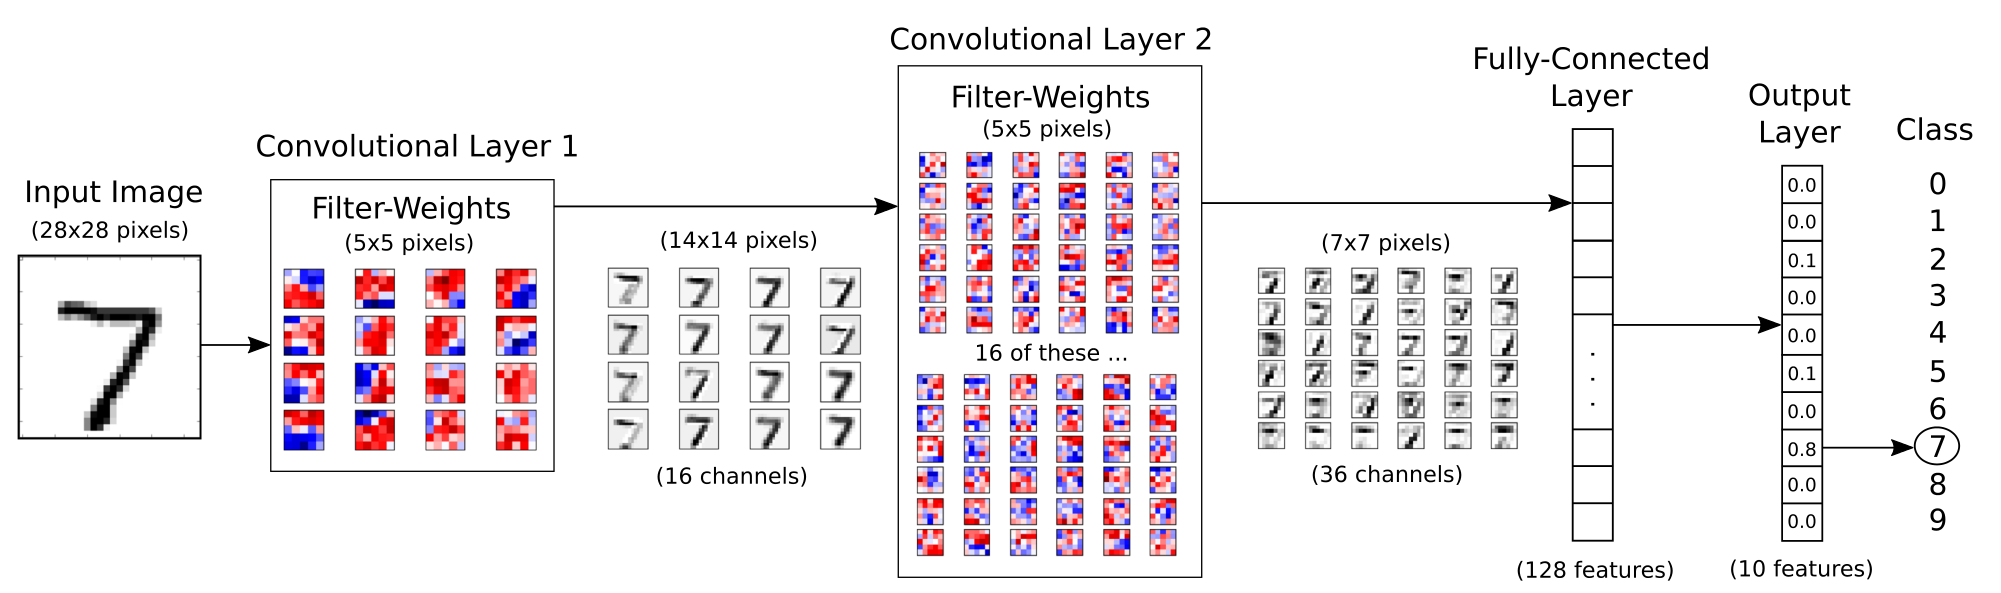
\includegraphics{data/images/02_network_flowchart.png}
\caption{Flowchart}
\end{figure}

    \hypertarget{Prep-and-Process}{}
PREPARATION AND PRE-PROCESSING

Imports

Now that we are a few lessons in, we have removed a portion of redundant
code in order to minimize the time it takes to read each lesson.

If you need to review it or make changes, it is in the data folder
provided with these lessons.

    \begin{Verbatim}[commandchars=\\\{\}]
{\color{incolor}In [{\color{incolor}1}]:} \PY{o}{\PYZpc{}}\PY{k}{run} data/shared\PYZus{}code.py
\end{Verbatim}


    \begin{Verbatim}[commandchars=\\\{\}]
C:\textbackslash{}Users\textbackslash{}Reasonable\textbackslash{}Anaconda3\textbackslash{}lib\textbackslash{}site-packages\textbackslash{}h5py\textbackslash{}\_\_init\_\_.py:34: FutureWarning: Conversion of the second argument of issubdtype from `float` to `np.floating` is deprecated. In future, it will be treated as `np.float64 == np.dtype(float).type`.
  from .\_conv import register\_converters as \_register\_converters

    \end{Verbatim}

    \begin{Verbatim}[commandchars=\\\{\}]

Preparing MNIST Dataset

Extracting data/MNIST/train-images-idx3-ubyte.gz
Extracting data/MNIST/train-labels-idx1-ubyte.gz
Extracting data/MNIST/t10k-images-idx3-ubyte.gz
Extracting data/MNIST/t10k-labels-idx1-ubyte.gz

Size of:
- Training-set:		55000
- Test-set:		10000
- Validation-set:	5000

Testing 'plot\_images()' Method

    \end{Verbatim}

    \begin{center}
    \adjustimage{max size={0.9\linewidth}{0.9\paperheight}}{output_4_2.png}
    \end{center}
    { \hspace*{\fill} \\}
    
    \begin{Verbatim}[commandchars=\\\{\}]
WARNING:tensorflow:From D:\textbackslash{}OneDrive\textbackslash{}Projects\textbackslash{}GitRepositories\textbackslash{}cooking-dough-with-tensorflow\textbackslash{}data\textbackslash{}shared\_code.py:90: calling argmax (from tensorflow.python.ops.math\_ops) with dimension is deprecated and will be removed in a future version.
Instructions for updating:
Use the `axis` argument instead

    \end{Verbatim}

    We need to import several things from Keras. Note the long
import-statements below. Hopefully it will be possible to write shorter
and more elegant lines in the future.

    \begin{Verbatim}[commandchars=\\\{\}]
{\color{incolor}In [{\color{incolor}2}]:} \PY{c+c1}{\PYZsh{} from tf.keras.models import Sequential    \PYZsh{} This does not work!}
        
        \PY{k+kn}{import} \PY{n+nn}{tensorflow}\PY{n+nn}{.}\PY{n+nn}{python}\PY{n+nn}{.}\PY{n+nn}{keras}
        \PY{k+kn}{from} \PY{n+nn}{tensorflow}\PY{n+nn}{.}\PY{n+nn}{python}\PY{n+nn}{.}\PY{n+nn}{keras}\PY{n+nn}{.}\PY{n+nn}{models} \PY{k}{import} \PY{n}{Sequential}
        \PY{k+kn}{from} \PY{n+nn}{tensorflow}\PY{n+nn}{.}\PY{n+nn}{python}\PY{n+nn}{.}\PY{n+nn}{keras}\PY{n+nn}{.}\PY{n+nn}{layers} \PY{k}{import} \PY{n}{InputLayer}\PY{p}{,} \PY{n}{Input}
        \PY{k+kn}{from} \PY{n+nn}{tensorflow}\PY{n+nn}{.}\PY{n+nn}{python}\PY{n+nn}{.}\PY{n+nn}{keras}\PY{n+nn}{.}\PY{n+nn}{layers} \PY{k}{import} \PY{n}{Reshape}\PY{p}{,} \PY{n}{MaxPooling2D}
        \PY{k+kn}{from} \PY{n+nn}{tensorflow}\PY{n+nn}{.}\PY{n+nn}{python}\PY{n+nn}{.}\PY{n+nn}{keras}\PY{n+nn}{.}\PY{n+nn}{layers} \PY{k}{import} \PY{n}{Conv2D}\PY{p}{,} \PY{n}{Dense}\PY{p}{,} \PY{n}{Flatten}
\end{Verbatim}


    This was developed using Python 3.6 (Anaconda) and TensorFlow version:

    \begin{Verbatim}[commandchars=\\\{\}]
{\color{incolor}In [{\color{incolor}3}]:} \PY{n}{tf}\PY{o}{.}\PY{n}{keras}\PY{o}{.}\PY{n}{\PYZus{}\PYZus{}version\PYZus{}\PYZus{}}
\end{Verbatim}


\begin{Verbatim}[commandchars=\\\{\}]
{\color{outcolor}Out[{\color{outcolor}3}]:} '2.1.3-tf'
\end{Verbatim}
            
    Helper-Function to Plot Example Errors

Function for plotting examples of images from the test-set that have
been mis-classified.

    \begin{Verbatim}[commandchars=\\\{\}]
{\color{incolor}In [{\color{incolor}4}]:} \PY{k}{def} \PY{n+nf}{plot\PYZus{}example\PYZus{}errors}\PY{p}{(}\PY{n}{cls\PYZus{}pred}\PY{p}{)}\PY{p}{:}
            \PY{c+c1}{\PYZsh{} cls\PYZus{}pred is an array of the predicted class\PYZhy{}number for}
            \PY{c+c1}{\PYZsh{} all images in the test\PYZhy{}set.}
        
            \PY{c+c1}{\PYZsh{} Boolean array whether the predicted class is incorrect.}
            \PY{n}{incorrect} \PY{o}{=} \PY{p}{(}\PY{n}{cls\PYZus{}pred} \PY{o}{!=} \PY{n}{data}\PY{o}{.}\PY{n}{test}\PY{o}{.}\PY{n}{cls}\PY{p}{)}
        
            \PY{c+c1}{\PYZsh{} Get the images from the test\PYZhy{}set that have been}
            \PY{c+c1}{\PYZsh{} incorrectly classified.}
            \PY{n}{images} \PY{o}{=} \PY{n}{data}\PY{o}{.}\PY{n}{test}\PY{o}{.}\PY{n}{images}\PY{p}{[}\PY{n}{incorrect}\PY{p}{]}
            
            \PY{c+c1}{\PYZsh{} Get the predicted classes for those images.}
            \PY{n}{cls\PYZus{}pred} \PY{o}{=} \PY{n}{cls\PYZus{}pred}\PY{p}{[}\PY{n}{incorrect}\PY{p}{]}
        
            \PY{c+c1}{\PYZsh{} Get the true classes for those images.}
            \PY{n}{cls\PYZus{}true} \PY{o}{=} \PY{n}{data}\PY{o}{.}\PY{n}{test}\PY{o}{.}\PY{n}{cls}\PY{p}{[}\PY{n}{incorrect}\PY{p}{]}
            
            \PY{c+c1}{\PYZsh{} Plot the first 9 images.}
            \PY{n}{plot\PYZus{}images}\PY{p}{(}\PY{n}{images}\PY{o}{=}\PY{n}{images}\PY{p}{[}\PY{l+m+mi}{0}\PY{p}{:}\PY{l+m+mi}{9}\PY{p}{]}\PY{p}{,}
                        \PY{n}{cls\PYZus{}true}\PY{o}{=}\PY{n}{cls\PYZus{}true}\PY{p}{[}\PY{l+m+mi}{0}\PY{p}{:}\PY{l+m+mi}{9}\PY{p}{]}\PY{p}{,}
                        \PY{n}{cls\PYZus{}pred}\PY{o}{=}\PY{n}{cls\PYZus{}pred}\PY{p}{[}\PY{l+m+mi}{0}\PY{p}{:}\PY{l+m+mi}{9}\PY{p}{]}\PY{p}{)}
\end{Verbatim}


    \hypertarget{Keras-API}{}
KERAS API

This is how the Convolutional Neural Network was implemented in Tutorial
\#03 using the PrettyTensor API. It is shown here for easy comparison to
the Keras implementation below.

    \begin{Verbatim}[commandchars=\\\{\}]
{\color{incolor}In [{\color{incolor}5}]:} \PY{k}{if} \PY{k+kc}{False}\PY{p}{:}
            \PY{n}{x\PYZus{}pretty} \PY{o}{=} \PY{n}{pt}\PY{o}{.}\PY{n}{wrap}\PY{p}{(}\PY{n}{x\PYZus{}image}\PY{p}{)}
        
            \PY{k}{with} \PY{n}{pt}\PY{o}{.}\PY{n}{defaults\PYZus{}scope}\PY{p}{(}\PY{n}{activation\PYZus{}fn}\PY{o}{=}\PY{n}{tf}\PY{o}{.}\PY{n}{nn}\PY{o}{.}\PY{n}{relu}\PY{p}{)}\PY{p}{:}
                \PY{n}{y\PYZus{}pred}\PY{p}{,} \PY{n}{loss} \PY{o}{=} \PY{n}{x\PYZus{}pretty}\PY{o}{.}\PYZbs{}
                    \PY{n}{conv2d}\PY{p}{(}\PY{n}{kernel}\PY{o}{=}\PY{l+m+mi}{5}\PY{p}{,} \PY{n}{depth}\PY{o}{=}\PY{l+m+mi}{16}\PY{p}{,} \PY{n}{name}\PY{o}{=}\PY{l+s+s1}{\PYZsq{}}\PY{l+s+s1}{layer\PYZus{}conv1}\PY{l+s+s1}{\PYZsq{}}\PY{p}{)}\PY{o}{.}\PYZbs{}
                    \PY{n}{max\PYZus{}pool}\PY{p}{(}\PY{n}{kernel}\PY{o}{=}\PY{l+m+mi}{2}\PY{p}{,} \PY{n}{stride}\PY{o}{=}\PY{l+m+mi}{2}\PY{p}{)}\PY{o}{.}\PYZbs{}
                    \PY{n}{conv2d}\PY{p}{(}\PY{n}{kernel}\PY{o}{=}\PY{l+m+mi}{5}\PY{p}{,} \PY{n}{depth}\PY{o}{=}\PY{l+m+mi}{36}\PY{p}{,} \PY{n}{name}\PY{o}{=}\PY{l+s+s1}{\PYZsq{}}\PY{l+s+s1}{layer\PYZus{}conv2}\PY{l+s+s1}{\PYZsq{}}\PY{p}{)}\PY{o}{.}\PYZbs{}
                    \PY{n}{max\PYZus{}pool}\PY{p}{(}\PY{n}{kernel}\PY{o}{=}\PY{l+m+mi}{2}\PY{p}{,} \PY{n}{stride}\PY{o}{=}\PY{l+m+mi}{2}\PY{p}{)}\PY{o}{.}\PYZbs{}
                    \PY{n}{flatten}\PY{p}{(}\PY{p}{)}\PY{o}{.}\PYZbs{}
                    \PY{n}{fully\PYZus{}connected}\PY{p}{(}\PY{n}{size}\PY{o}{=}\PY{l+m+mi}{128}\PY{p}{,} \PY{n}{name}\PY{o}{=}\PY{l+s+s1}{\PYZsq{}}\PY{l+s+s1}{layer\PYZus{}fc1}\PY{l+s+s1}{\PYZsq{}}\PY{p}{)}\PY{o}{.}\PYZbs{}
                    \PY{n}{softmax\PYZus{}classifier}\PY{p}{(}\PY{n}{num\PYZus{}classes}\PY{o}{=}\PY{n}{num\PYZus{}classes}\PY{p}{,} \PY{n}{labels}\PY{o}{=}\PY{n}{y\PYZus{}true}\PY{p}{)}
\end{Verbatim}


    \hypertarget{Sequential-Model}{}
SEQUENTIAL MODEL

The Keras API has two modes of constructing Neural Networks. The
simplest is the Sequential Model which only allows for the layers to be
added in sequence.

    \begin{Verbatim}[commandchars=\\\{\}]
{\color{incolor}In [{\color{incolor}6}]:} \PY{c+c1}{\PYZsh{} Start construction of the Keras Sequential model.}
        \PY{n}{model} \PY{o}{=} \PY{n}{Sequential}\PY{p}{(}\PY{p}{)}
        
        \PY{c+c1}{\PYZsh{} Add an input layer which is similar to a feed\PYZus{}dict in TensorFlow.}
        \PY{c+c1}{\PYZsh{} Note that the input\PYZhy{}shape must be a tuple containing the image\PYZhy{}size.}
        \PY{n}{model}\PY{o}{.}\PY{n}{add}\PY{p}{(}\PY{n}{InputLayer}\PY{p}{(}\PY{n}{input\PYZus{}shape}\PY{o}{=}\PY{p}{(}\PY{n}{img\PYZus{}size\PYZus{}flat}\PY{p}{,}\PY{p}{)}\PY{p}{)}\PY{p}{)}
        
        \PY{c+c1}{\PYZsh{} The input is a flattened array with 784 elements,}
        \PY{c+c1}{\PYZsh{} but the convolutional layers expect images with shape (28, 28, 1)}
        \PY{n}{model}\PY{o}{.}\PY{n}{add}\PY{p}{(}\PY{n}{Reshape}\PY{p}{(}\PY{n}{img\PYZus{}shape\PYZus{}full}\PY{p}{)}\PY{p}{)}
        
        \PY{c+c1}{\PYZsh{} First convolutional layer with ReLU\PYZhy{}activation and max\PYZhy{}pooling.}
        \PY{n}{model}\PY{o}{.}\PY{n}{add}\PY{p}{(}\PY{n}{Conv2D}\PY{p}{(}\PY{n}{kernel\PYZus{}size}\PY{o}{=}\PY{l+m+mi}{5}\PY{p}{,} \PY{n}{strides}\PY{o}{=}\PY{l+m+mi}{1}\PY{p}{,} \PY{n}{filters}\PY{o}{=}\PY{l+m+mi}{16}\PY{p}{,} \PY{n}{padding}\PY{o}{=}\PY{l+s+s1}{\PYZsq{}}\PY{l+s+s1}{same}\PY{l+s+s1}{\PYZsq{}}\PY{p}{,}
                         \PY{n}{activation}\PY{o}{=}\PY{l+s+s1}{\PYZsq{}}\PY{l+s+s1}{relu}\PY{l+s+s1}{\PYZsq{}}\PY{p}{,} \PY{n}{name}\PY{o}{=}\PY{l+s+s1}{\PYZsq{}}\PY{l+s+s1}{layer\PYZus{}conv1}\PY{l+s+s1}{\PYZsq{}}\PY{p}{)}\PY{p}{)}
        \PY{n}{model}\PY{o}{.}\PY{n}{add}\PY{p}{(}\PY{n}{MaxPooling2D}\PY{p}{(}\PY{n}{pool\PYZus{}size}\PY{o}{=}\PY{l+m+mi}{2}\PY{p}{,} \PY{n}{strides}\PY{o}{=}\PY{l+m+mi}{2}\PY{p}{)}\PY{p}{)}
        
        \PY{c+c1}{\PYZsh{} Second convolutional layer with ReLU\PYZhy{}activation and max\PYZhy{}pooling.}
        \PY{n}{model}\PY{o}{.}\PY{n}{add}\PY{p}{(}\PY{n}{Conv2D}\PY{p}{(}\PY{n}{kernel\PYZus{}size}\PY{o}{=}\PY{l+m+mi}{5}\PY{p}{,} \PY{n}{strides}\PY{o}{=}\PY{l+m+mi}{1}\PY{p}{,} \PY{n}{filters}\PY{o}{=}\PY{l+m+mi}{36}\PY{p}{,} \PY{n}{padding}\PY{o}{=}\PY{l+s+s1}{\PYZsq{}}\PY{l+s+s1}{same}\PY{l+s+s1}{\PYZsq{}}\PY{p}{,}
                         \PY{n}{activation}\PY{o}{=}\PY{l+s+s1}{\PYZsq{}}\PY{l+s+s1}{relu}\PY{l+s+s1}{\PYZsq{}}\PY{p}{,} \PY{n}{name}\PY{o}{=}\PY{l+s+s1}{\PYZsq{}}\PY{l+s+s1}{layer\PYZus{}conv2}\PY{l+s+s1}{\PYZsq{}}\PY{p}{)}\PY{p}{)}
        \PY{n}{model}\PY{o}{.}\PY{n}{add}\PY{p}{(}\PY{n}{MaxPooling2D}\PY{p}{(}\PY{n}{pool\PYZus{}size}\PY{o}{=}\PY{l+m+mi}{2}\PY{p}{,} \PY{n}{strides}\PY{o}{=}\PY{l+m+mi}{2}\PY{p}{)}\PY{p}{)}
        
        \PY{c+c1}{\PYZsh{} Flatten the 4\PYZhy{}rank output of the convolutional layers}
        \PY{c+c1}{\PYZsh{} to 2\PYZhy{}rank that can be input to a fully\PYZhy{}connected / dense layer.}
        \PY{n}{model}\PY{o}{.}\PY{n}{add}\PY{p}{(}\PY{n}{Flatten}\PY{p}{(}\PY{p}{)}\PY{p}{)}
        
        \PY{c+c1}{\PYZsh{} First fully\PYZhy{}connected / dense layer with ReLU\PYZhy{}activation.}
        \PY{n}{model}\PY{o}{.}\PY{n}{add}\PY{p}{(}\PY{n}{Dense}\PY{p}{(}\PY{l+m+mi}{128}\PY{p}{,} \PY{n}{activation}\PY{o}{=}\PY{l+s+s1}{\PYZsq{}}\PY{l+s+s1}{relu}\PY{l+s+s1}{\PYZsq{}}\PY{p}{)}\PY{p}{)}
        
        \PY{c+c1}{\PYZsh{} Last fully\PYZhy{}connected / dense layer with softmax\PYZhy{}activation}
        \PY{c+c1}{\PYZsh{} for use in classification.}
        \PY{n}{model}\PY{o}{.}\PY{n}{add}\PY{p}{(}\PY{n}{Dense}\PY{p}{(}\PY{n}{num\PYZus{}classes}\PY{p}{,} \PY{n}{activation}\PY{o}{=}\PY{l+s+s1}{\PYZsq{}}\PY{l+s+s1}{softmax}\PY{l+s+s1}{\PYZsq{}}\PY{p}{)}\PY{p}{)}
\end{Verbatim}


    Model Compilation

The Neural Network has now been defined and must be finalized by adding
a loss-function, optimizer and performance metrics. This is called model
"compilation" in Keras.

We can either define the optimizer using a string, or if we want more
control of its parameters then we need to instantiate an object. For
example, we can set the learning-rate.

    \begin{Verbatim}[commandchars=\\\{\}]
{\color{incolor}In [{\color{incolor}7}]:} \PY{k+kn}{from} \PY{n+nn}{tensorflow}\PY{n+nn}{.}\PY{n+nn}{python}\PY{n+nn}{.}\PY{n+nn}{keras}\PY{n+nn}{.}\PY{n+nn}{optimizers} \PY{k}{import} \PY{n}{Adam}
        
        \PY{n}{optimizer} \PY{o}{=} \PY{n}{Adam}\PY{p}{(}\PY{n}{lr}\PY{o}{=}\PY{l+m+mf}{1e\PYZhy{}3}\PY{p}{)}
\end{Verbatim}


    For a classification-problem such as MNIST which has 10 possible
classes, we need to use the loss-function called
\texttt{categorical\_crossentropy}. The performance metric we are
interested in is the classification accuracy.

    \begin{Verbatim}[commandchars=\\\{\}]
{\color{incolor}In [{\color{incolor}8}]:} \PY{n}{model}\PY{o}{.}\PY{n}{compile}\PY{p}{(}\PY{n}{optimizer}\PY{o}{=}\PY{n}{optimizer}\PY{p}{,}
                      \PY{n}{loss}\PY{o}{=}\PY{l+s+s1}{\PYZsq{}}\PY{l+s+s1}{categorical\PYZus{}crossentropy}\PY{l+s+s1}{\PYZsq{}}\PY{p}{,}
                      \PY{n}{metrics}\PY{o}{=}\PY{p}{[}\PY{l+s+s1}{\PYZsq{}}\PY{l+s+s1}{accuracy}\PY{l+s+s1}{\PYZsq{}}\PY{p}{]}\PY{p}{)}
\end{Verbatim}


    Training

Now that the model has been fully defined with loss-function and
optimizer, we can train it. This function takes numpy-arrays and
performs the given number of training epochs using the given batch-size.
An epoch is one full use of the entire training-set. So for 10 epochs we
would iterate randomly over the entire training-set 10 times.

    \begin{Verbatim}[commandchars=\\\{\}]
{\color{incolor}In [{\color{incolor}9}]:} \PY{n}{model}\PY{o}{.}\PY{n}{fit}\PY{p}{(}\PY{n}{x}\PY{o}{=}\PY{n}{data}\PY{o}{.}\PY{n}{train}\PY{o}{.}\PY{n}{images}\PY{p}{,}
                  \PY{n}{y}\PY{o}{=}\PY{n}{data}\PY{o}{.}\PY{n}{train}\PY{o}{.}\PY{n}{labels}\PY{p}{,}
                  \PY{n}{epochs}\PY{o}{=}\PY{l+m+mi}{1}\PY{p}{,} \PY{n}{batch\PYZus{}size}\PY{o}{=}\PY{l+m+mi}{128}\PY{p}{)}
\end{Verbatim}


    \begin{Verbatim}[commandchars=\\\{\}]
Epoch 1/1
55000/55000 [==============================]55000/55000 [==============================] - 36s 659us/step - loss: 0.2132 - acc: 0.9367


    \end{Verbatim}

\begin{Verbatim}[commandchars=\\\{\}]
{\color{outcolor}Out[{\color{outcolor}9}]:} <tensorflow.python.keras.\_impl.keras.callbacks.History at 0x24980354fd0>
\end{Verbatim}
            
    Evaluation

Now that the model has been trained we can test its performance on the
test-set. This also uses numpy-arrays as input.

    \begin{Verbatim}[commandchars=\\\{\}]
{\color{incolor}In [{\color{incolor}10}]:} \PY{n}{result} \PY{o}{=} \PY{n}{model}\PY{o}{.}\PY{n}{evaluate}\PY{p}{(}\PY{n}{x}\PY{o}{=}\PY{n}{data}\PY{o}{.}\PY{n}{test}\PY{o}{.}\PY{n}{images}\PY{p}{,}
                                 \PY{n}{y}\PY{o}{=}\PY{n}{data}\PY{o}{.}\PY{n}{test}\PY{o}{.}\PY{n}{labels}\PY{p}{)}
\end{Verbatim}


    \begin{Verbatim}[commandchars=\\\{\}]
10000/10000 [==============================]10000/10000 [==============================] - 3s 302us/step


    \end{Verbatim}

    We can print all the performance metrics for the test-set.

    \begin{Verbatim}[commandchars=\\\{\}]
{\color{incolor}In [{\color{incolor}11}]:} \PY{k}{for} \PY{n}{name}\PY{p}{,} \PY{n}{value} \PY{o+ow}{in} \PY{n+nb}{zip}\PY{p}{(}\PY{n}{model}\PY{o}{.}\PY{n}{metrics\PYZus{}names}\PY{p}{,} \PY{n}{result}\PY{p}{)}\PY{p}{:}
             \PY{n+nb}{print}\PY{p}{(}\PY{n}{name}\PY{p}{,} \PY{n}{value}\PY{p}{)}
\end{Verbatim}


    \begin{Verbatim}[commandchars=\\\{\}]
loss 0.0606757159546949
acc 0.9811

    \end{Verbatim}

    Or we can just print the classification accuracy.

    \begin{Verbatim}[commandchars=\\\{\}]
{\color{incolor}In [{\color{incolor}12}]:} \PY{n+nb}{print}\PY{p}{(}\PY{l+s+s2}{\PYZdq{}}\PY{l+s+si}{\PYZob{}0\PYZcb{}}\PY{l+s+s2}{: }\PY{l+s+si}{\PYZob{}1:.2\PYZpc{}\PYZcb{}}\PY{l+s+s2}{\PYZdq{}}\PY{o}{.}\PY{n}{format}\PY{p}{(}\PY{n}{model}\PY{o}{.}\PY{n}{metrics\PYZus{}names}\PY{p}{[}\PY{l+m+mi}{1}\PY{p}{]}\PY{p}{,} \PY{n}{result}\PY{p}{[}\PY{l+m+mi}{1}\PY{p}{]}\PY{p}{)}\PY{p}{)}
\end{Verbatim}


    \begin{Verbatim}[commandchars=\\\{\}]
acc: 98.11\%

    \end{Verbatim}

    Prediction

We can also predict the classification for new images. We will just use
some images from the test-set but you could load your own images into
numpy arrays and use those instead.

    \begin{Verbatim}[commandchars=\\\{\}]
{\color{incolor}In [{\color{incolor}13}]:} \PY{n}{images} \PY{o}{=} \PY{n}{data}\PY{o}{.}\PY{n}{test}\PY{o}{.}\PY{n}{images}\PY{p}{[}\PY{l+m+mi}{0}\PY{p}{:}\PY{l+m+mi}{9}\PY{p}{]}
\end{Verbatim}


    These are the true class-number for those images. This is only used when
plotting the images.

    \begin{Verbatim}[commandchars=\\\{\}]
{\color{incolor}In [{\color{incolor}14}]:} \PY{n}{cls\PYZus{}true} \PY{o}{=} \PY{n}{data}\PY{o}{.}\PY{n}{test}\PY{o}{.}\PY{n}{cls}\PY{p}{[}\PY{l+m+mi}{0}\PY{p}{:}\PY{l+m+mi}{9}\PY{p}{]}
\end{Verbatim}


    Get the predicted classes as One-Hot encoded arrays.

    \begin{Verbatim}[commandchars=\\\{\}]
{\color{incolor}In [{\color{incolor}15}]:} \PY{n}{y\PYZus{}pred} \PY{o}{=} \PY{n}{model}\PY{o}{.}\PY{n}{predict}\PY{p}{(}\PY{n}{x}\PY{o}{=}\PY{n}{images}\PY{p}{)}
\end{Verbatim}


    Get the predicted classes as integers.

    \begin{Verbatim}[commandchars=\\\{\}]
{\color{incolor}In [{\color{incolor}16}]:} \PY{n}{cls\PYZus{}pred} \PY{o}{=} \PY{n}{np}\PY{o}{.}\PY{n}{argmax}\PY{p}{(}\PY{n}{y\PYZus{}pred}\PY{p}{,}\PY{n}{axis}\PY{o}{=}\PY{l+m+mi}{1}\PY{p}{)}
\end{Verbatim}


    \begin{Verbatim}[commandchars=\\\{\}]
{\color{incolor}In [{\color{incolor}17}]:} \PY{n}{plot\PYZus{}images}\PY{p}{(}\PY{n}{images}\PY{o}{=}\PY{n}{images}\PY{p}{,}
                     \PY{n}{cls\PYZus{}true}\PY{o}{=}\PY{n}{cls\PYZus{}true}\PY{p}{,}
                     \PY{n}{cls\PYZus{}pred}\PY{o}{=}\PY{n}{cls\PYZus{}pred}\PY{p}{)}
\end{Verbatim}


    \begin{center}
    \adjustimage{max size={0.9\linewidth}{0.9\paperheight}}{output_35_0.png}
    \end{center}
    { \hspace*{\fill} \\}
    
    Examples of Mis-Classified Images

We can plot some examples of mis-classified images from the test-set.

First we get the predicted classes for all the images in the test-set:

    \begin{Verbatim}[commandchars=\\\{\}]
{\color{incolor}In [{\color{incolor}18}]:} \PY{n}{y\PYZus{}pred} \PY{o}{=} \PY{n}{model}\PY{o}{.}\PY{n}{predict}\PY{p}{(}\PY{n}{x}\PY{o}{=}\PY{n}{data}\PY{o}{.}\PY{n}{test}\PY{o}{.}\PY{n}{images}\PY{p}{)}
\end{Verbatim}


    Then we convert the predicted class-numbers from One-Hot encoded arrays
to integers.

    \begin{Verbatim}[commandchars=\\\{\}]
{\color{incolor}In [{\color{incolor}19}]:} \PY{n}{cls\PYZus{}pred} \PY{o}{=} \PY{n}{np}\PY{o}{.}\PY{n}{argmax}\PY{p}{(}\PY{n}{y\PYZus{}pred}\PY{p}{,}\PY{n}{axis}\PY{o}{=}\PY{l+m+mi}{1}\PY{p}{)}
\end{Verbatim}


    Plot some of the mis-classified images.

    \begin{Verbatim}[commandchars=\\\{\}]
{\color{incolor}In [{\color{incolor}20}]:} \PY{n}{plot\PYZus{}example\PYZus{}errors}\PY{p}{(}\PY{n}{cls\PYZus{}pred}\PY{p}{)}
\end{Verbatim}


    \begin{center}
    \adjustimage{max size={0.9\linewidth}{0.9\paperheight}}{output_41_0.png}
    \end{center}
    { \hspace*{\fill} \\}
    
    \hypertarget{Functional-Model}{}
FUNCTIONAL MODEL

The Keras API can also be used to construct more complicated networks
using the Functional Model. This may look a little confusing at first,
because each call to the Keras API will create and return an instance
that is itself callable. It is not clear whether it is a function or an
object - but we can call it as if it is a function. This allows us to
build computational graphs that are more complex than the Sequential
Model allows.

    \begin{Verbatim}[commandchars=\\\{\}]
{\color{incolor}In [{\color{incolor}21}]:} \PY{c+c1}{\PYZsh{} Create an input layer which is similar to a feed\PYZus{}dict in TensorFlow.}
         \PY{c+c1}{\PYZsh{} Note that the input\PYZhy{}shape must be a tuple containing the image\PYZhy{}size.}
         \PY{n}{inputs} \PY{o}{=} \PY{n}{Input}\PY{p}{(}\PY{n}{shape}\PY{o}{=}\PY{p}{(}\PY{n}{img\PYZus{}size\PYZus{}flat}\PY{p}{,}\PY{p}{)}\PY{p}{)}
         
         \PY{c+c1}{\PYZsh{} Variable used for building the Neural Network.}
         \PY{n}{net} \PY{o}{=} \PY{n}{inputs}
         
         \PY{c+c1}{\PYZsh{} The input is an image as a flattened array with 784 elements.}
         \PY{c+c1}{\PYZsh{} But the convolutional layers expect images with shape (28, 28, 1)}
         \PY{n}{net} \PY{o}{=} \PY{n}{Reshape}\PY{p}{(}\PY{n}{img\PYZus{}shape\PYZus{}full}\PY{p}{)}\PY{p}{(}\PY{n}{net}\PY{p}{)}
         
         \PY{c+c1}{\PYZsh{} First convolutional layer with ReLU\PYZhy{}activation and max\PYZhy{}pooling.}
         \PY{n}{net} \PY{o}{=} \PY{n}{Conv2D}\PY{p}{(}\PY{n}{kernel\PYZus{}size}\PY{o}{=}\PY{l+m+mi}{5}\PY{p}{,} \PY{n}{strides}\PY{o}{=}\PY{l+m+mi}{1}\PY{p}{,} \PY{n}{filters}\PY{o}{=}\PY{l+m+mi}{16}\PY{p}{,} \PY{n}{padding}\PY{o}{=}\PY{l+s+s1}{\PYZsq{}}\PY{l+s+s1}{same}\PY{l+s+s1}{\PYZsq{}}\PY{p}{,}
                      \PY{n}{activation}\PY{o}{=}\PY{l+s+s1}{\PYZsq{}}\PY{l+s+s1}{relu}\PY{l+s+s1}{\PYZsq{}}\PY{p}{,} \PY{n}{name}\PY{o}{=}\PY{l+s+s1}{\PYZsq{}}\PY{l+s+s1}{layer\PYZus{}conv1}\PY{l+s+s1}{\PYZsq{}}\PY{p}{)}\PY{p}{(}\PY{n}{net}\PY{p}{)}
         \PY{n}{net} \PY{o}{=} \PY{n}{MaxPooling2D}\PY{p}{(}\PY{n}{pool\PYZus{}size}\PY{o}{=}\PY{l+m+mi}{2}\PY{p}{,} \PY{n}{strides}\PY{o}{=}\PY{l+m+mi}{2}\PY{p}{)}\PY{p}{(}\PY{n}{net}\PY{p}{)}
         
         \PY{c+c1}{\PYZsh{} Second convolutional layer with ReLU\PYZhy{}activation and max\PYZhy{}pooling.}
         \PY{n}{net} \PY{o}{=} \PY{n}{Conv2D}\PY{p}{(}\PY{n}{kernel\PYZus{}size}\PY{o}{=}\PY{l+m+mi}{5}\PY{p}{,} \PY{n}{strides}\PY{o}{=}\PY{l+m+mi}{1}\PY{p}{,} \PY{n}{filters}\PY{o}{=}\PY{l+m+mi}{36}\PY{p}{,} \PY{n}{padding}\PY{o}{=}\PY{l+s+s1}{\PYZsq{}}\PY{l+s+s1}{same}\PY{l+s+s1}{\PYZsq{}}\PY{p}{,}
                      \PY{n}{activation}\PY{o}{=}\PY{l+s+s1}{\PYZsq{}}\PY{l+s+s1}{relu}\PY{l+s+s1}{\PYZsq{}}\PY{p}{,} \PY{n}{name}\PY{o}{=}\PY{l+s+s1}{\PYZsq{}}\PY{l+s+s1}{layer\PYZus{}conv2}\PY{l+s+s1}{\PYZsq{}}\PY{p}{)}\PY{p}{(}\PY{n}{net}\PY{p}{)}
         \PY{n}{net} \PY{o}{=} \PY{n}{MaxPooling2D}\PY{p}{(}\PY{n}{pool\PYZus{}size}\PY{o}{=}\PY{l+m+mi}{2}\PY{p}{,} \PY{n}{strides}\PY{o}{=}\PY{l+m+mi}{2}\PY{p}{)}\PY{p}{(}\PY{n}{net}\PY{p}{)}
         
         \PY{c+c1}{\PYZsh{} Flatten the output of the conv\PYZhy{}layer from 4\PYZhy{}dim to 2\PYZhy{}dim.}
         \PY{n}{net} \PY{o}{=} \PY{n}{Flatten}\PY{p}{(}\PY{p}{)}\PY{p}{(}\PY{n}{net}\PY{p}{)}
         
         \PY{c+c1}{\PYZsh{} First fully\PYZhy{}connected / dense layer with ReLU\PYZhy{}activation.}
         \PY{n}{net} \PY{o}{=} \PY{n}{Dense}\PY{p}{(}\PY{l+m+mi}{128}\PY{p}{,} \PY{n}{activation}\PY{o}{=}\PY{l+s+s1}{\PYZsq{}}\PY{l+s+s1}{relu}\PY{l+s+s1}{\PYZsq{}}\PY{p}{)}\PY{p}{(}\PY{n}{net}\PY{p}{)}
         
         \PY{c+c1}{\PYZsh{} Last fully\PYZhy{}connected / dense layer with softmax\PYZhy{}activation}
         \PY{c+c1}{\PYZsh{} so it can be used for classification.}
         \PY{n}{net} \PY{o}{=} \PY{n}{Dense}\PY{p}{(}\PY{n}{num\PYZus{}classes}\PY{p}{,} \PY{n}{activation}\PY{o}{=}\PY{l+s+s1}{\PYZsq{}}\PY{l+s+s1}{softmax}\PY{l+s+s1}{\PYZsq{}}\PY{p}{)}\PY{p}{(}\PY{n}{net}\PY{p}{)}
         
         \PY{c+c1}{\PYZsh{} Output of the Neural Network.}
         \PY{n}{outputs} \PY{o}{=} \PY{n}{net}
\end{Verbatim}


    Model Compilation

We have now defined the architecture of the model with its input and
output. We now have to create a Keras model and compile it with a
loss-function and optimizer, so it is ready for training.

    \begin{Verbatim}[commandchars=\\\{\}]
{\color{incolor}In [{\color{incolor}22}]:} \PY{k+kn}{from} \PY{n+nn}{tensorflow}\PY{n+nn}{.}\PY{n+nn}{python}\PY{n+nn}{.}\PY{n+nn}{keras}\PY{n+nn}{.}\PY{n+nn}{models} \PY{k}{import} \PY{n}{Model}
\end{Verbatim}


    Create a new instance of the Keras Functional Model. We give it the
inputs and outputs of the Convolutional Neural Network that we
constructed above.

    \begin{Verbatim}[commandchars=\\\{\}]
{\color{incolor}In [{\color{incolor}23}]:} \PY{n}{model2} \PY{o}{=} \PY{n}{Model}\PY{p}{(}\PY{n}{inputs}\PY{o}{=}\PY{n}{inputs}\PY{p}{,} \PY{n}{outputs}\PY{o}{=}\PY{n}{outputs}\PY{p}{)}
\end{Verbatim}


    Compile the Keras model using the \texttt{rmsprop} optimizer and with a
loss-function for multiple categories. The only performance metric we
are interested in is the classification accuracy, but you could use a
list of metrics here.

    \begin{Verbatim}[commandchars=\\\{\}]
{\color{incolor}In [{\color{incolor}24}]:} \PY{n}{model2}\PY{o}{.}\PY{n}{compile}\PY{p}{(}\PY{n}{optimizer}\PY{o}{=}\PY{l+s+s1}{\PYZsq{}}\PY{l+s+s1}{rmsprop}\PY{l+s+s1}{\PYZsq{}}\PY{p}{,}
                        \PY{n}{loss}\PY{o}{=}\PY{l+s+s1}{\PYZsq{}}\PY{l+s+s1}{categorical\PYZus{}crossentropy}\PY{l+s+s1}{\PYZsq{}}\PY{p}{,}
                        \PY{n}{metrics}\PY{o}{=}\PY{p}{[}\PY{l+s+s1}{\PYZsq{}}\PY{l+s+s1}{accuracy}\PY{l+s+s1}{\PYZsq{}}\PY{p}{]}\PY{p}{)}
\end{Verbatim}


    Training

The model has now been defined and compiled so it can be trained using
the same \texttt{fit()} function as used in the Sequential Model above.
This also takes numpy-arrays as input.

    \begin{Verbatim}[commandchars=\\\{\}]
{\color{incolor}In [{\color{incolor}25}]:} \PY{n}{model2}\PY{o}{.}\PY{n}{fit}\PY{p}{(}\PY{n}{x}\PY{o}{=}\PY{n}{data}\PY{o}{.}\PY{n}{train}\PY{o}{.}\PY{n}{images}\PY{p}{,}
                    \PY{n}{y}\PY{o}{=}\PY{n}{data}\PY{o}{.}\PY{n}{train}\PY{o}{.}\PY{n}{labels}\PY{p}{,}
                    \PY{n}{epochs}\PY{o}{=}\PY{l+m+mi}{1}\PY{p}{,} \PY{n}{batch\PYZus{}size}\PY{o}{=}\PY{l+m+mi}{128}\PY{p}{)}
\end{Verbatim}


    \begin{Verbatim}[commandchars=\\\{\}]
Epoch 1/1
55000/55000 [==============================]55000/55000 [==============================] - 36s 646us/step - loss: 0.2070 - acc: 0.9350


    \end{Verbatim}

\begin{Verbatim}[commandchars=\\\{\}]
{\color{outcolor}Out[{\color{outcolor}25}]:} <tensorflow.python.keras.\_impl.keras.callbacks.History at 0x249800d8320>
\end{Verbatim}
            
    Evaluation

Once the model has been trained we can evaluate its performance on the
test-set. This is the same syntax as for the Sequential Model.

    \begin{Verbatim}[commandchars=\\\{\}]
{\color{incolor}In [{\color{incolor}26}]:} \PY{n}{result} \PY{o}{=} \PY{n}{model2}\PY{o}{.}\PY{n}{evaluate}\PY{p}{(}\PY{n}{x}\PY{o}{=}\PY{n}{data}\PY{o}{.}\PY{n}{test}\PY{o}{.}\PY{n}{images}\PY{p}{,}
                                  \PY{n}{y}\PY{o}{=}\PY{n}{data}\PY{o}{.}\PY{n}{test}\PY{o}{.}\PY{n}{labels}\PY{p}{)}
\end{Verbatim}


    \begin{Verbatim}[commandchars=\\\{\}]
10000/10000 [==============================]10000/10000 [==============================] - 3s 300us/step


    \end{Verbatim}

    The result is a list of values, containing the loss-value and all the
metrics we defined when we compiled the model. Note that 'accuracy' is
now called 'acc' which is a small inconsistency.

    \begin{Verbatim}[commandchars=\\\{\}]
{\color{incolor}In [{\color{incolor}27}]:} \PY{k}{for} \PY{n}{name}\PY{p}{,} \PY{n}{value} \PY{o+ow}{in} \PY{n+nb}{zip}\PY{p}{(}\PY{n}{model}\PY{o}{.}\PY{n}{metrics\PYZus{}names}\PY{p}{,} \PY{n}{result}\PY{p}{)}\PY{p}{:}
             \PY{n+nb}{print}\PY{p}{(}\PY{n}{name}\PY{p}{,} \PY{n}{value}\PY{p}{)}
\end{Verbatim}


    \begin{Verbatim}[commandchars=\\\{\}]
loss 0.07508188281003386
acc 0.9764

    \end{Verbatim}

    We can also print the classification accuracy as a percentage:

    \begin{Verbatim}[commandchars=\\\{\}]
{\color{incolor}In [{\color{incolor}28}]:} \PY{n+nb}{print}\PY{p}{(}\PY{l+s+s2}{\PYZdq{}}\PY{l+s+si}{\PYZob{}0\PYZcb{}}\PY{l+s+s2}{: }\PY{l+s+si}{\PYZob{}1:.2\PYZpc{}\PYZcb{}}\PY{l+s+s2}{\PYZdq{}}\PY{o}{.}\PY{n}{format}\PY{p}{(}\PY{n}{model}\PY{o}{.}\PY{n}{metrics\PYZus{}names}\PY{p}{[}\PY{l+m+mi}{1}\PY{p}{]}\PY{p}{,} \PY{n}{result}\PY{p}{[}\PY{l+m+mi}{1}\PY{p}{]}\PY{p}{)}\PY{p}{)}
\end{Verbatim}


    \begin{Verbatim}[commandchars=\\\{\}]
acc: 97.64\%

    \end{Verbatim}

    Examples of Mis-Classified Images

We can plot some examples of mis-classified images from the test-set.

First we get the predicted classes for all the images in the test-set:

    \begin{Verbatim}[commandchars=\\\{\}]
{\color{incolor}In [{\color{incolor}29}]:} \PY{n}{y\PYZus{}pred} \PY{o}{=} \PY{n}{model2}\PY{o}{.}\PY{n}{predict}\PY{p}{(}\PY{n}{x}\PY{o}{=}\PY{n}{data}\PY{o}{.}\PY{n}{test}\PY{o}{.}\PY{n}{images}\PY{p}{)}
\end{Verbatim}


    Then we convert the predicted class-numbers from One-Hot encoded arrays
to integers.

    \begin{Verbatim}[commandchars=\\\{\}]
{\color{incolor}In [{\color{incolor}30}]:} \PY{n}{cls\PYZus{}pred} \PY{o}{=} \PY{n}{np}\PY{o}{.}\PY{n}{argmax}\PY{p}{(}\PY{n}{y\PYZus{}pred}\PY{p}{,} \PY{n}{axis}\PY{o}{=}\PY{l+m+mi}{1}\PY{p}{)}
\end{Verbatim}


    Plot some of the mis-classified images.

    \begin{Verbatim}[commandchars=\\\{\}]
{\color{incolor}In [{\color{incolor}31}]:} \PY{n}{plot\PYZus{}example\PYZus{}errors}\PY{p}{(}\PY{n}{cls\PYZus{}pred}\PY{p}{)}
\end{Verbatim}


    \begin{center}
    \adjustimage{max size={0.9\linewidth}{0.9\paperheight}}{output_63_0.png}
    \end{center}
    { \hspace*{\fill} \\}
    
    Save and Load Model

NOTE

\begin{quote}
\begin{itemize}
\tightlist
\item
  You need to install \texttt{h5py} for this to work!
\item
  Tutorial \#04 was about saving and restoring the weights of a model
  using native TensorFlow code.
\item
  It was an absolutely horrible API! Fortunately, Keras makes this very
  easy.
\end{itemize}
\end{quote}

This is the file-path where we want to save the Keras model.

    \begin{Verbatim}[commandchars=\\\{\}]
{\color{incolor}In [{\color{incolor}32}]:} \PY{n}{path\PYZus{}model} \PY{o}{=} \PY{l+s+s1}{\PYZsq{}}\PY{l+s+s1}{models/model.keras}\PY{l+s+s1}{\PYZsq{}}
\end{Verbatim}


    Saving a Keras model with the trained weights is then just a single
function call, as it should be.

    \begin{Verbatim}[commandchars=\\\{\}]
{\color{incolor}In [{\color{incolor}33}]:} \PY{n}{model2}\PY{o}{.}\PY{n}{save}\PY{p}{(}\PY{n}{path\PYZus{}model}\PY{p}{)}
\end{Verbatim}


    Delete the model from memory so we are sure it is no longer used.

    \begin{Verbatim}[commandchars=\\\{\}]
{\color{incolor}In [{\color{incolor}34}]:} \PY{k}{del} \PY{n}{model2}
\end{Verbatim}


    We need to import this Keras function for loading the model.

    \begin{Verbatim}[commandchars=\\\{\}]
{\color{incolor}In [{\color{incolor}35}]:} \PY{k+kn}{from} \PY{n+nn}{tensorflow}\PY{n+nn}{.}\PY{n+nn}{python}\PY{n+nn}{.}\PY{n+nn}{keras}\PY{n+nn}{.}\PY{n+nn}{models} \PY{k}{import} \PY{n}{load\PYZus{}model}
\end{Verbatim}


    Loading the model is then just a single function-call, as it should be.

    \begin{Verbatim}[commandchars=\\\{\}]
{\color{incolor}In [{\color{incolor}36}]:} \PY{n}{model3} \PY{o}{=} \PY{n}{load\PYZus{}model}\PY{p}{(}\PY{n}{path\PYZus{}model}\PY{p}{)}
\end{Verbatim}


    We can then use the model again e.g. to make predictions. We get the
first 9 images from the test-set and their true class-numbers.

    \begin{Verbatim}[commandchars=\\\{\}]
{\color{incolor}In [{\color{incolor}37}]:} \PY{n}{images} \PY{o}{=} \PY{n}{data}\PY{o}{.}\PY{n}{test}\PY{o}{.}\PY{n}{images}\PY{p}{[}\PY{l+m+mi}{0}\PY{p}{:}\PY{l+m+mi}{9}\PY{p}{]}
\end{Verbatim}


    \begin{Verbatim}[commandchars=\\\{\}]
{\color{incolor}In [{\color{incolor}38}]:} \PY{n}{cls\PYZus{}true} \PY{o}{=} \PY{n}{data}\PY{o}{.}\PY{n}{test}\PY{o}{.}\PY{n}{cls}\PY{p}{[}\PY{l+m+mi}{0}\PY{p}{:}\PY{l+m+mi}{9}\PY{p}{]}
\end{Verbatim}


    We then use the restored model to predict the class-numbers for those
images.

    \begin{Verbatim}[commandchars=\\\{\}]
{\color{incolor}In [{\color{incolor}39}]:} \PY{n}{y\PYZus{}pred} \PY{o}{=} \PY{n}{model3}\PY{o}{.}\PY{n}{predict}\PY{p}{(}\PY{n}{x}\PY{o}{=}\PY{n}{images}\PY{p}{)}
\end{Verbatim}


    Get the class-numbers as integers.

    \begin{Verbatim}[commandchars=\\\{\}]
{\color{incolor}In [{\color{incolor}40}]:} \PY{n}{cls\PYZus{}pred} \PY{o}{=} \PY{n}{np}\PY{o}{.}\PY{n}{argmax}\PY{p}{(}\PY{n}{y\PYZus{}pred}\PY{p}{,} \PY{n}{axis}\PY{o}{=}\PY{l+m+mi}{1}\PY{p}{)}
\end{Verbatim}


    Plot the images with their true and predicted class-numbers.

    \begin{Verbatim}[commandchars=\\\{\}]
{\color{incolor}In [{\color{incolor}41}]:} \PY{n}{plot\PYZus{}images}\PY{p}{(}\PY{n}{images}\PY{o}{=}\PY{n}{images}\PY{p}{,}
                     \PY{n}{cls\PYZus{}pred}\PY{o}{=}\PY{n}{cls\PYZus{}pred}\PY{p}{,}
                     \PY{n}{cls\PYZus{}true}\PY{o}{=}\PY{n}{cls\PYZus{}true}\PY{p}{)}
\end{Verbatim}


    \begin{center}
    \adjustimage{max size={0.9\linewidth}{0.9\paperheight}}{output_82_0.png}
    \end{center}
    { \hspace*{\fill} \\}
    
    \hypertarget{Visualization-Weights-Outputs}{}
VISUALIZATION OF LAYER WEIGHTS AND OUTPUTS

    Helper-Function for Plotting Convolutional Weights

    \begin{Verbatim}[commandchars=\\\{\}]
{\color{incolor}In [{\color{incolor}42}]:} \PY{k}{def} \PY{n+nf}{plot\PYZus{}conv\PYZus{}weights}\PY{p}{(}\PY{n}{weights}\PY{p}{,} \PY{n}{input\PYZus{}channel}\PY{o}{=}\PY{l+m+mi}{0}\PY{p}{)}\PY{p}{:}
             \PY{c+c1}{\PYZsh{} Get the lowest and highest values for the weights.}
             \PY{c+c1}{\PYZsh{} This is used to correct the colour intensity across}
             \PY{c+c1}{\PYZsh{} the images so they can be compared with each other.}
             \PY{n}{w\PYZus{}min} \PY{o}{=} \PY{n}{np}\PY{o}{.}\PY{n}{min}\PY{p}{(}\PY{n}{weights}\PY{p}{)}
             \PY{n}{w\PYZus{}max} \PY{o}{=} \PY{n}{np}\PY{o}{.}\PY{n}{max}\PY{p}{(}\PY{n}{weights}\PY{p}{)}
         
             \PY{c+c1}{\PYZsh{} Number of filters used in the conv. layer.}
             \PY{n}{num\PYZus{}filters} \PY{o}{=} \PY{n}{weights}\PY{o}{.}\PY{n}{shape}\PY{p}{[}\PY{l+m+mi}{3}\PY{p}{]}
         
             \PY{c+c1}{\PYZsh{} Number of grids to plot.}
             \PY{c+c1}{\PYZsh{} Rounded\PYZhy{}up, square\PYZhy{}root of the number of filters.}
             \PY{n}{num\PYZus{}grids} \PY{o}{=} \PY{n}{math}\PY{o}{.}\PY{n}{ceil}\PY{p}{(}\PY{n}{math}\PY{o}{.}\PY{n}{sqrt}\PY{p}{(}\PY{n}{num\PYZus{}filters}\PY{p}{)}\PY{p}{)}
             
             \PY{c+c1}{\PYZsh{} Create figure with a grid of sub\PYZhy{}plots.}
             \PY{n}{fig}\PY{p}{,} \PY{n}{axes} \PY{o}{=} \PY{n}{plt}\PY{o}{.}\PY{n}{subplots}\PY{p}{(}\PY{n}{num\PYZus{}grids}\PY{p}{,} \PY{n}{num\PYZus{}grids}\PY{p}{)}
         
             \PY{c+c1}{\PYZsh{} Plot all the filter\PYZhy{}weights.}
             \PY{k}{for} \PY{n}{i}\PY{p}{,} \PY{n}{ax} \PY{o+ow}{in} \PY{n+nb}{enumerate}\PY{p}{(}\PY{n}{axes}\PY{o}{.}\PY{n}{flat}\PY{p}{)}\PY{p}{:}
                 \PY{c+c1}{\PYZsh{} Only plot the valid filter\PYZhy{}weights.}
                 \PY{k}{if} \PY{n}{i}\PY{o}{\PYZlt{}}\PY{n}{num\PYZus{}filters}\PY{p}{:}
                     \PY{c+c1}{\PYZsh{} Get the weights for the i\PYZsq{}th filter of the input channel.}
                     \PY{c+c1}{\PYZsh{} See new\PYZus{}conv\PYZus{}layer() for details on the format}
                     \PY{c+c1}{\PYZsh{} of this 4\PYZhy{}dim tensor.}
                     \PY{n}{img} \PY{o}{=} \PY{n}{weights}\PY{p}{[}\PY{p}{:}\PY{p}{,} \PY{p}{:}\PY{p}{,} \PY{n}{input\PYZus{}channel}\PY{p}{,} \PY{n}{i}\PY{p}{]}
         
                     \PY{c+c1}{\PYZsh{} Plot image.}
                     \PY{n}{ax}\PY{o}{.}\PY{n}{imshow}\PY{p}{(}\PY{n}{img}\PY{p}{,} \PY{n}{vmin}\PY{o}{=}\PY{n}{w\PYZus{}min}\PY{p}{,} \PY{n}{vmax}\PY{o}{=}\PY{n}{w\PYZus{}max}\PY{p}{,}
                               \PY{n}{interpolation}\PY{o}{=}\PY{l+s+s1}{\PYZsq{}}\PY{l+s+s1}{nearest}\PY{l+s+s1}{\PYZsq{}}\PY{p}{,} \PY{n}{cmap}\PY{o}{=}\PY{l+s+s1}{\PYZsq{}}\PY{l+s+s1}{seismic}\PY{l+s+s1}{\PYZsq{}}\PY{p}{)}
                 
                 \PY{c+c1}{\PYZsh{} Remove ticks from the plot.}
                 \PY{n}{ax}\PY{o}{.}\PY{n}{set\PYZus{}xticks}\PY{p}{(}\PY{p}{[}\PY{p}{]}\PY{p}{)}
                 \PY{n}{ax}\PY{o}{.}\PY{n}{set\PYZus{}yticks}\PY{p}{(}\PY{p}{[}\PY{p}{]}\PY{p}{)}
             
             \PY{c+c1}{\PYZsh{} Ensure the plot is shown correctly with multiple plots}
             \PY{c+c1}{\PYZsh{} in a single Notebook cell.}
             \PY{n}{plt}\PY{o}{.}\PY{n}{show}\PY{p}{(}\PY{p}{)}
\end{Verbatim}


    \hypertarget{Get-Layers}{}
GET LAYERS

Keras has a simple way of listing the layers in the model.

    \begin{Verbatim}[commandchars=\\\{\}]
{\color{incolor}In [{\color{incolor}43}]:} \PY{n}{model3}\PY{o}{.}\PY{n}{summary}\PY{p}{(}\PY{p}{)}
\end{Verbatim}


    \begin{Verbatim}[commandchars=\\\{\}]
\_\_\_\_\_\_\_\_\_\_\_\_\_\_\_\_\_\_\_\_\_\_\_\_\_\_\_\_\_\_\_\_\_\_\_\_\_\_\_\_\_\_\_\_\_\_\_\_\_\_\_\_\_\_\_\_\_\_\_\_\_\_\_\_\_
Layer (type)                 Output Shape              Param \#   
=================================================================
input\_2 (InputLayer)         (None, 784)               0         
\_\_\_\_\_\_\_\_\_\_\_\_\_\_\_\_\_\_\_\_\_\_\_\_\_\_\_\_\_\_\_\_\_\_\_\_\_\_\_\_\_\_\_\_\_\_\_\_\_\_\_\_\_\_\_\_\_\_\_\_\_\_\_\_\_
reshape\_2 (Reshape)          (None, 28, 28, 1)         0         
\_\_\_\_\_\_\_\_\_\_\_\_\_\_\_\_\_\_\_\_\_\_\_\_\_\_\_\_\_\_\_\_\_\_\_\_\_\_\_\_\_\_\_\_\_\_\_\_\_\_\_\_\_\_\_\_\_\_\_\_\_\_\_\_\_
layer\_conv1 (Conv2D)         (None, 28, 28, 16)        416       
\_\_\_\_\_\_\_\_\_\_\_\_\_\_\_\_\_\_\_\_\_\_\_\_\_\_\_\_\_\_\_\_\_\_\_\_\_\_\_\_\_\_\_\_\_\_\_\_\_\_\_\_\_\_\_\_\_\_\_\_\_\_\_\_\_
max\_pooling2d\_3 (MaxPooling2 (None, 14, 14, 16)        0         
\_\_\_\_\_\_\_\_\_\_\_\_\_\_\_\_\_\_\_\_\_\_\_\_\_\_\_\_\_\_\_\_\_\_\_\_\_\_\_\_\_\_\_\_\_\_\_\_\_\_\_\_\_\_\_\_\_\_\_\_\_\_\_\_\_
layer\_conv2 (Conv2D)         (None, 14, 14, 36)        14436     
\_\_\_\_\_\_\_\_\_\_\_\_\_\_\_\_\_\_\_\_\_\_\_\_\_\_\_\_\_\_\_\_\_\_\_\_\_\_\_\_\_\_\_\_\_\_\_\_\_\_\_\_\_\_\_\_\_\_\_\_\_\_\_\_\_
max\_pooling2d\_4 (MaxPooling2 (None, 7, 7, 36)          0         
\_\_\_\_\_\_\_\_\_\_\_\_\_\_\_\_\_\_\_\_\_\_\_\_\_\_\_\_\_\_\_\_\_\_\_\_\_\_\_\_\_\_\_\_\_\_\_\_\_\_\_\_\_\_\_\_\_\_\_\_\_\_\_\_\_
flatten\_2 (Flatten)          (None, 1764)              0         
\_\_\_\_\_\_\_\_\_\_\_\_\_\_\_\_\_\_\_\_\_\_\_\_\_\_\_\_\_\_\_\_\_\_\_\_\_\_\_\_\_\_\_\_\_\_\_\_\_\_\_\_\_\_\_\_\_\_\_\_\_\_\_\_\_
dense\_3 (Dense)              (None, 128)               225920    
\_\_\_\_\_\_\_\_\_\_\_\_\_\_\_\_\_\_\_\_\_\_\_\_\_\_\_\_\_\_\_\_\_\_\_\_\_\_\_\_\_\_\_\_\_\_\_\_\_\_\_\_\_\_\_\_\_\_\_\_\_\_\_\_\_
dense\_4 (Dense)              (None, 10)                1290      
=================================================================
Total params: 242,062
Trainable params: 242,062
Non-trainable params: 0
\_\_\_\_\_\_\_\_\_\_\_\_\_\_\_\_\_\_\_\_\_\_\_\_\_\_\_\_\_\_\_\_\_\_\_\_\_\_\_\_\_\_\_\_\_\_\_\_\_\_\_\_\_\_\_\_\_\_\_\_\_\_\_\_\_

    \end{Verbatim}

    We count the indices to get the layers we want.

The input-layer has index 0.

    \begin{Verbatim}[commandchars=\\\{\}]
{\color{incolor}In [{\color{incolor}44}]:} \PY{n}{layer\PYZus{}input} \PY{o}{=} \PY{n}{model3}\PY{o}{.}\PY{n}{layers}\PY{p}{[}\PY{l+m+mi}{0}\PY{p}{]}
\end{Verbatim}


    The first convolutional layer has index 2.

    \begin{Verbatim}[commandchars=\\\{\}]
{\color{incolor}In [{\color{incolor}45}]:} \PY{n}{layer\PYZus{}conv1} \PY{o}{=} \PY{n}{model3}\PY{o}{.}\PY{n}{layers}\PY{p}{[}\PY{l+m+mi}{2}\PY{p}{]}
         \PY{n}{layer\PYZus{}conv1}
\end{Verbatim}


\begin{Verbatim}[commandchars=\\\{\}]
{\color{outcolor}Out[{\color{outcolor}45}]:} <tensorflow.python.keras.\_impl.keras.layers.convolutional.Conv2D at 0x24982f6bf60>
\end{Verbatim}
            
    The second convolutional layer has index 4.

    \begin{Verbatim}[commandchars=\\\{\}]
{\color{incolor}In [{\color{incolor}46}]:} \PY{n}{layer\PYZus{}conv2} \PY{o}{=} \PY{n}{model3}\PY{o}{.}\PY{n}{layers}\PY{p}{[}\PY{l+m+mi}{4}\PY{p}{]}
\end{Verbatim}


    Convolutional Weights

Now that we have the layers we can easily get their weights.

    \begin{Verbatim}[commandchars=\\\{\}]
{\color{incolor}In [{\color{incolor}47}]:} \PY{n}{weights\PYZus{}conv1} \PY{o}{=} \PY{n}{layer\PYZus{}conv1}\PY{o}{.}\PY{n}{get\PYZus{}weights}\PY{p}{(}\PY{p}{)}\PY{p}{[}\PY{l+m+mi}{0}\PY{p}{]}
\end{Verbatim}


    This gives us a 4-rank tensor.

    \begin{Verbatim}[commandchars=\\\{\}]
{\color{incolor}In [{\color{incolor}48}]:} \PY{n}{weights\PYZus{}conv1}\PY{o}{.}\PY{n}{shape}
\end{Verbatim}


\begin{Verbatim}[commandchars=\\\{\}]
{\color{outcolor}Out[{\color{outcolor}48}]:} (5, 5, 1, 16)
\end{Verbatim}
            
    Plot the weights using the helper-function from above.

    \begin{Verbatim}[commandchars=\\\{\}]
{\color{incolor}In [{\color{incolor}49}]:} \PY{n}{plot\PYZus{}conv\PYZus{}weights}\PY{p}{(}\PY{n}{weights}\PY{o}{=}\PY{n}{weights\PYZus{}conv1}\PY{p}{,} \PY{n}{input\PYZus{}channel}\PY{o}{=}\PY{l+m+mi}{0}\PY{p}{)}
\end{Verbatim}


    \begin{center}
    \adjustimage{max size={0.9\linewidth}{0.9\paperheight}}{output_99_0.png}
    \end{center}
    { \hspace*{\fill} \\}
    
    We can also get the weights for the second convolutional layer and plot
them.

    \begin{Verbatim}[commandchars=\\\{\}]
{\color{incolor}In [{\color{incolor}50}]:} \PY{n}{weights\PYZus{}conv2} \PY{o}{=} \PY{n}{layer\PYZus{}conv2}\PY{o}{.}\PY{n}{get\PYZus{}weights}\PY{p}{(}\PY{p}{)}\PY{p}{[}\PY{l+m+mi}{0}\PY{p}{]}
\end{Verbatim}


    \begin{Verbatim}[commandchars=\\\{\}]
{\color{incolor}In [{\color{incolor}51}]:} \PY{n}{plot\PYZus{}conv\PYZus{}weights}\PY{p}{(}\PY{n}{weights}\PY{o}{=}\PY{n}{weights\PYZus{}conv2}\PY{p}{,} \PY{n}{input\PYZus{}channel}\PY{o}{=}\PY{l+m+mi}{0}\PY{p}{)}
\end{Verbatim}


    \begin{center}
    \adjustimage{max size={0.9\linewidth}{0.9\paperheight}}{output_102_0.png}
    \end{center}
    { \hspace*{\fill} \\}
    
    Helper-Function for Plotting the Output of a Convolutional Layer

    \begin{Verbatim}[commandchars=\\\{\}]
{\color{incolor}In [{\color{incolor}52}]:} \PY{k}{def} \PY{n+nf}{plot\PYZus{}conv\PYZus{}output}\PY{p}{(}\PY{n}{values}\PY{p}{)}\PY{p}{:}
             \PY{c+c1}{\PYZsh{} Number of filters used in the conv. layer.}
             \PY{n}{num\PYZus{}filters} \PY{o}{=} \PY{n}{values}\PY{o}{.}\PY{n}{shape}\PY{p}{[}\PY{l+m+mi}{3}\PY{p}{]}
         
             \PY{c+c1}{\PYZsh{} Number of grids to plot.}
             \PY{c+c1}{\PYZsh{} Rounded\PYZhy{}up, square\PYZhy{}root of the number of filters.}
             \PY{n}{num\PYZus{}grids} \PY{o}{=} \PY{n}{math}\PY{o}{.}\PY{n}{ceil}\PY{p}{(}\PY{n}{math}\PY{o}{.}\PY{n}{sqrt}\PY{p}{(}\PY{n}{num\PYZus{}filters}\PY{p}{)}\PY{p}{)}
             
             \PY{c+c1}{\PYZsh{} Create figure with a grid of sub\PYZhy{}plots.}
             \PY{n}{fig}\PY{p}{,} \PY{n}{axes} \PY{o}{=} \PY{n}{plt}\PY{o}{.}\PY{n}{subplots}\PY{p}{(}\PY{n}{num\PYZus{}grids}\PY{p}{,} \PY{n}{num\PYZus{}grids}\PY{p}{)}
         
             \PY{c+c1}{\PYZsh{} Plot the output images of all the filters.}
             \PY{k}{for} \PY{n}{i}\PY{p}{,} \PY{n}{ax} \PY{o+ow}{in} \PY{n+nb}{enumerate}\PY{p}{(}\PY{n}{axes}\PY{o}{.}\PY{n}{flat}\PY{p}{)}\PY{p}{:}
                 \PY{c+c1}{\PYZsh{} Only plot the images for valid filters.}
                 \PY{k}{if} \PY{n}{i} \PY{o}{\PYZlt{}} \PY{n}{num\PYZus{}filters}\PY{p}{:}
                     \PY{c+c1}{\PYZsh{} Get the output image of using the i\PYZsq{}th filter.}
                     \PY{n}{img} \PY{o}{=} \PY{n}{values}\PY{p}{[}\PY{l+m+mi}{0}\PY{p}{,} \PY{p}{:}\PY{p}{,} \PY{p}{:}\PY{p}{,} \PY{n}{i}\PY{p}{]}
         
                     \PY{c+c1}{\PYZsh{} Plot image.}
                     \PY{n}{ax}\PY{o}{.}\PY{n}{imshow}\PY{p}{(}\PY{n}{img}\PY{p}{,} \PY{n}{interpolation}\PY{o}{=}\PY{l+s+s1}{\PYZsq{}}\PY{l+s+s1}{nearest}\PY{l+s+s1}{\PYZsq{}}\PY{p}{,} \PY{n}{cmap}\PY{o}{=}\PY{l+s+s1}{\PYZsq{}}\PY{l+s+s1}{binary}\PY{l+s+s1}{\PYZsq{}}\PY{p}{)}
                 
                 \PY{c+c1}{\PYZsh{} Remove ticks from the plot.}
                 \PY{n}{ax}\PY{o}{.}\PY{n}{set\PYZus{}xticks}\PY{p}{(}\PY{p}{[}\PY{p}{]}\PY{p}{)}
                 \PY{n}{ax}\PY{o}{.}\PY{n}{set\PYZus{}yticks}\PY{p}{(}\PY{p}{[}\PY{p}{]}\PY{p}{)}
             
             \PY{c+c1}{\PYZsh{} Ensure the plot is shown correctly with multiple plots}
             \PY{c+c1}{\PYZsh{} in a single Notebook cell.}
             \PY{n}{plt}\PY{o}{.}\PY{n}{show}\PY{p}{(}\PY{p}{)}
\end{Verbatim}


    Input Image

Helper-function for plotting a single image.

    \begin{Verbatim}[commandchars=\\\{\}]
{\color{incolor}In [{\color{incolor}53}]:} \PY{k}{def} \PY{n+nf}{plot\PYZus{}image}\PY{p}{(}\PY{n}{image}\PY{p}{)}\PY{p}{:}
             \PY{n}{plt}\PY{o}{.}\PY{n}{imshow}\PY{p}{(}\PY{n}{image}\PY{o}{.}\PY{n}{reshape}\PY{p}{(}\PY{n}{img\PYZus{}shape}\PY{p}{)}\PY{p}{,}
                        \PY{n}{interpolation}\PY{o}{=}\PY{l+s+s1}{\PYZsq{}}\PY{l+s+s1}{nearest}\PY{l+s+s1}{\PYZsq{}}\PY{p}{,}
                        \PY{n}{cmap}\PY{o}{=}\PY{l+s+s1}{\PYZsq{}}\PY{l+s+s1}{binary}\PY{l+s+s1}{\PYZsq{}}\PY{p}{)}
         
             \PY{n}{plt}\PY{o}{.}\PY{n}{show}\PY{p}{(}\PY{p}{)}
\end{Verbatim}


    Plot an image from the test-set which will be used as an example below.

    \begin{Verbatim}[commandchars=\\\{\}]
{\color{incolor}In [{\color{incolor}54}]:} \PY{n}{image1} \PY{o}{=} \PY{n}{data}\PY{o}{.}\PY{n}{test}\PY{o}{.}\PY{n}{images}\PY{p}{[}\PY{l+m+mi}{0}\PY{p}{]}
         \PY{n}{plot\PYZus{}image}\PY{p}{(}\PY{n}{image1}\PY{p}{)}
\end{Verbatim}


    \begin{center}
    \adjustimage{max size={0.9\linewidth}{0.9\paperheight}}{output_108_0.png}
    \end{center}
    { \hspace*{\fill} \\}
    
    \hypertarget{Output-Convolutional-Layer-Method-1}{}
OUTPUT OF CONVOLUTIONAL LAYER - METHOD 1

There are different ways of getting the output of a layer in a Keras
model. This method uses a so-called K-function which turns a part of the
Keras model into a function.

    \begin{Verbatim}[commandchars=\\\{\}]
{\color{incolor}In [{\color{incolor}55}]:} \PY{k+kn}{from} \PY{n+nn}{tensorflow}\PY{n+nn}{.}\PY{n+nn}{python}\PY{n+nn}{.}\PY{n+nn}{keras} \PY{k}{import} \PY{n}{backend} \PY{k}{as} \PY{n}{K}
\end{Verbatim}


    \begin{Verbatim}[commandchars=\\\{\}]
{\color{incolor}In [{\color{incolor}56}]:} \PY{n}{output\PYZus{}conv1} \PY{o}{=} \PY{n}{K}\PY{o}{.}\PY{n}{function}\PY{p}{(}\PY{n}{inputs}\PY{o}{=}\PY{p}{[}\PY{n}{layer\PYZus{}input}\PY{o}{.}\PY{n}{input}\PY{p}{]}\PY{p}{,}
                                   \PY{n}{outputs}\PY{o}{=}\PY{p}{[}\PY{n}{layer\PYZus{}conv1}\PY{o}{.}\PY{n}{output}\PY{p}{]}\PY{p}{)}
\end{Verbatim}


    We can then call this function with the input image. Note that the image
is wrapped in two lists because the function expects an array of that
dimensionality. Likewise, the function returns an array with one more
dimensionality than we want so we just take the first element.

    \begin{Verbatim}[commandchars=\\\{\}]
{\color{incolor}In [{\color{incolor}57}]:} \PY{n}{layer\PYZus{}output1} \PY{o}{=} \PY{n}{output\PYZus{}conv1}\PY{p}{(}\PY{p}{[}\PY{p}{[}\PY{n}{image1}\PY{p}{]}\PY{p}{]}\PY{p}{)}\PY{p}{[}\PY{l+m+mi}{0}\PY{p}{]}
         \PY{n}{layer\PYZus{}output1}\PY{o}{.}\PY{n}{shape}
\end{Verbatim}


\begin{Verbatim}[commandchars=\\\{\}]
{\color{outcolor}Out[{\color{outcolor}57}]:} (1, 28, 28, 16)
\end{Verbatim}
            
    We can then plot the output of all 16 channels of the convolutional
layer.

    \begin{Verbatim}[commandchars=\\\{\}]
{\color{incolor}In [{\color{incolor}58}]:} \PY{n}{plot\PYZus{}conv\PYZus{}output}\PY{p}{(}\PY{n}{values}\PY{o}{=}\PY{n}{layer\PYZus{}output1}\PY{p}{)}
\end{Verbatim}


    \begin{center}
    \adjustimage{max size={0.9\linewidth}{0.9\paperheight}}{output_115_0.png}
    \end{center}
    { \hspace*{\fill} \\}
    
    \hypertarget{Output-Convolutional-Layer-Method-2}{}
OUTPUT OF CONVOLUTIONAL LAYER - METHOD 2

Keras also has another method for getting the output of a layer inside
the model. This creates another Functional Model using the same input as
the original model, but the output is now taken from the convolutional
layer that we are interested in.

    \begin{Verbatim}[commandchars=\\\{\}]
{\color{incolor}In [{\color{incolor}59}]:} \PY{n}{output\PYZus{}conv2} \PY{o}{=} \PY{n}{Model}\PY{p}{(}\PY{n}{inputs}\PY{o}{=}\PY{n}{layer\PYZus{}input}\PY{o}{.}\PY{n}{input}\PY{p}{,}
                              \PY{n}{outputs}\PY{o}{=}\PY{n}{layer\PYZus{}conv2}\PY{o}{.}\PY{n}{output}\PY{p}{)}
\end{Verbatim}


    This creates a new model-object where we can call the typical Keras
functions. To get the output of the convoloutional layer we call the
\texttt{predict()} function with the input image.

    \begin{Verbatim}[commandchars=\\\{\}]
{\color{incolor}In [{\color{incolor}60}]:} \PY{n}{layer\PYZus{}output2} \PY{o}{=} \PY{n}{output\PYZus{}conv2}\PY{o}{.}\PY{n}{predict}\PY{p}{(}\PY{n}{np}\PY{o}{.}\PY{n}{array}\PY{p}{(}\PY{p}{[}\PY{n}{image1}\PY{p}{]}\PY{p}{)}\PY{p}{)}
         \PY{n}{layer\PYZus{}output2}\PY{o}{.}\PY{n}{shape}
\end{Verbatim}


\begin{Verbatim}[commandchars=\\\{\}]
{\color{outcolor}Out[{\color{outcolor}60}]:} (1, 14, 14, 36)
\end{Verbatim}
            
    We can then plot the images for all 36 channels.

    \begin{Verbatim}[commandchars=\\\{\}]
{\color{incolor}In [{\color{incolor}61}]:} \PY{n}{plot\PYZus{}conv\PYZus{}output}\PY{p}{(}\PY{n}{values}\PY{o}{=}\PY{n}{layer\PYZus{}output2}\PY{p}{)}
\end{Verbatim}


    \begin{center}
    \adjustimage{max size={0.9\linewidth}{0.9\paperheight}}{output_121_0.png}
    \end{center}
    { \hspace*{\fill} \\}
    
    \hypertarget{Summary}{}
SUMMARY

This tutorial showed how to use the so-called \emph{Keras API} for
easily building Convolutional Neural Networks in TensorFlow. Keras is by
far the most complete and best designed API for TensorFlow.

This tutorial also showed how to use Keras to save and load a model, as
well as getting the weights and outputs of convolutional layers.

It seems likely that Keras will be the standard API for TensorFlow in
the future, for the simple reason that is already very good and it is
constantly being improved. So it is recommended that you use Keras.

    \hypertarget{Challenge}{}
CHALLENGE

These are a few suggestions for exercises that may help improve your
skills with TensorFlow. It is important to get hands-on experience with
TensorFlow in order to learn how to use it properly.

You may want to backup this Notebook before making any changes.

\begin{itemize}
\tightlist
\item
  Train for more epochs. Does it improve the classification accuracy?
\item
  Change the activation function to sigmoid for some of the layers.
\item
  Can you find a simple way of changing the activation function for all
  the layers?
\item
  Plot the output of the max-pooling layers instead of the conv-layers.
\item
  Replace the 2x2 max-pooling layers with stride=2 in the convolutional
  layers. Is there a difference in classification accuracy? What if you
  optimize it again and again? The difference is random, so how would
  you measure if there really is a difference? What are the pros and
  cons of using max-pooling vs. stride in the conv-layer?
\item
  Change the parameters for the layers, e.g. the kernel, depth, size,
  etc. What is the difference in time usage and classification accuracy?
\item
  Add and remove some convolutional and fully-connected layers.
\item
  What is the simplest network you can design that still performs well?
\item
  Change the Functional Model so it has another convolutional layer that
  connects in parallel to the existing conv-layers before going into the
  dense layers.
\item
  Change the Functional Model so it outputs the predicted class both as
  a One-Hot encoded array and as an integer, so we don't have to use
  \texttt{numpy.argmax()} afterwards.
\item
  Remake the program yourself without looking too much at this
  source-code.
\item
  Explain to a friend how the program works.
\end{itemize}

    \hypertarget{Summary}{}
LICENSE (MIT)

Copyright (c) 2016-2017 by \href{http://www.hvass-labs.org/}{Magnus Erik
Hvass Pedersen}

Permission is hereby granted, free of charge, to any person obtaining a
copy of this software and associated documentation files (the
"Software"), to deal in the Software without restriction, including
without limitation the rights to use, copy, modify, merge, publish,
distribute, sublicense, and/or sell copies of the Software, and to
permit persons to whom the Software is furnished to do so, subject to
the following conditions:

The above copyright notice and this permission notice shall be included
in all copies or substantial portions of the Software.

THE SOFTWARE IS PROVIDED "AS IS", WITHOUT WARRANTY OF ANY KIND, EXPRESS
OR IMPLIED, INCLUDING BUT NOT LIMITED TO THE WARRANTIES OF
MERCHANTABILITY, FITNESS FOR A PARTICULAR PURPOSE AND NONINFRINGEMENT.
IN NO EVENT SHALL THE AUTHORS OR COPYRIGHT HOLDERS BE LIABLE FOR ANY
CLAIM, DAMAGES OR OTHER LIABILITY, WHETHER IN AN ACTION OF CONTRACT,
TORT OR OTHERWISE, ARISING FROM, OUT OF OR IN CONNECTION WITH THE
SOFTWARE OR THE USE OR OTHER DEALINGS IN THE SOFTWARE.


    % Add a bibliography block to the postdoc
    
    
    
    \end{document}
